\chapter{Reconstruction et identification des particules et objets}
\label{chap5}

Ce chapitre est consacré à la description des différentes méthodes de reconstruction et d'identification des particules et objets avec le détecteur CMS. Malgré la grande variété de particules produites lors des collisions proton-proton, seules quelques-unes sont stables à l'échelle du détecteur et peuvent être identifiées. Parmi celles-ci se trouvent les muons ($\mu^{\pm}$), les électrons (e$^{\pm}$), les hadrons chargés (p, $\pi^{\pm}$) et neutres (n, $\pi^0$), et les photons ($\gamma$). Chacune d'elles possède une signature qui lui est propre au sein de chaque sous-détecteur (fig. \ref{CMSslice}) et la combinaison de ces informations à travers l'algorithme du flux de particules, dont une présentation est donnée dans la première partie de ce chapitre, permet leur reconstruction.
Ces particules sont ensuite utilisées comme éléments de base pour la reconstruction d'autres particules ou d'objets plus complexes. Dans la suite, une présentation des méthodes permettant la reconstruction et l'identification des gerbes hadroniques (\textit{jets}) et de l'énergie transverse manquante sera donnée, ainsi qu'une partie dédiée au lepton tau, ce dernier étant l'objet clef de l'analyse réalisée dans cette thèse. 

\section{Algorithme du flux de particules (\textit{Particle Flow})}
\label{PF}

L'algorithme du flux de particules \cite{ThePFAlgo} se fonde sur la combinaison des informations de plusieurs sous-détecteurs pour identifier et reconstruire les particules produites lors des collisions. Le détecteur utilisant l'algorithme doit posséder au moins deux caractéristiques essentielles pour un fonctionnement optimal. La première repose sur un champ magnétique suffisamment fort ainsi qu'une bonne granularité des calorimètres afin d'éviter le recouvrement des dépôts d'énergie et assurer une bonne séparation entre hadrons neutres et chargés. La seconde repose sur la bonne performance du trajectographe et sur un faible budget de matière pour ne pas altérer la mesure des calorimètres. Dans le cas de CMS, ces aspects sont couverts par son trajectographe en silicium équipé de pixels et de bandes, l'excellente granularité de son calorimètre électromagnétique et la bonne hermicité de son calorimètre hadronique. L'aimant supraconducteur est placé à l'extérieur de ces éléments, ce qui permet une meilleure association entre les informations du trajectographe et des calorimètres. Enfin, les larges dernières couches de détection dédiées aux muons permettent une reconstruction et une identification optimale de ces derniers en complétant les informations du trajectographe. \\

\begin{figure}
\centering
    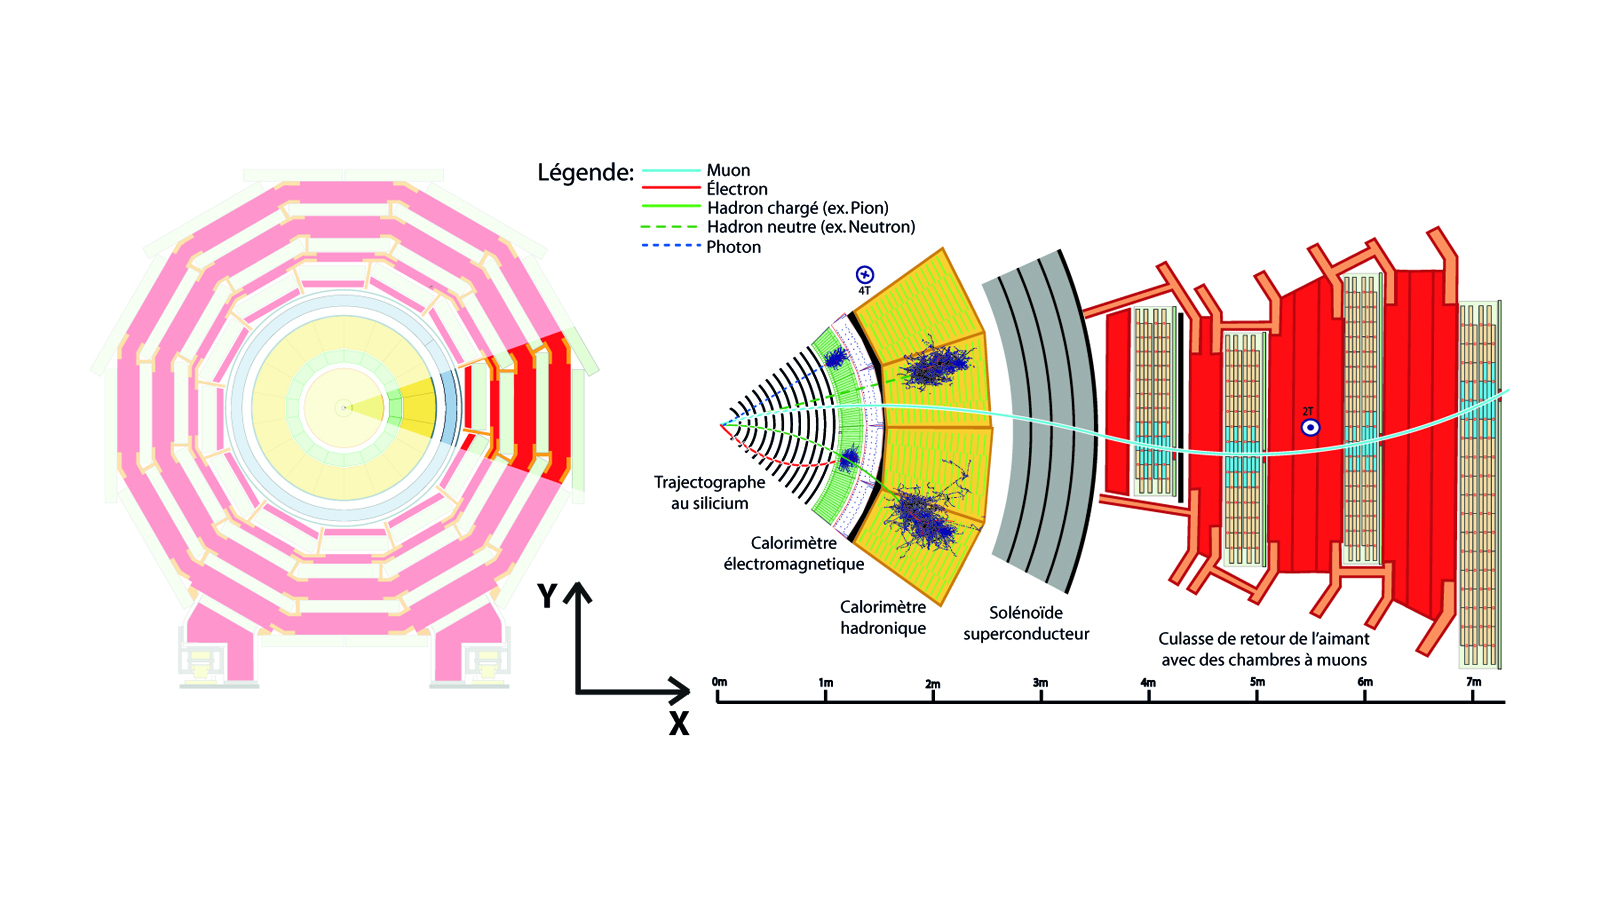
\includegraphics[scale=1.1]{Chapitre4/Images/CMSslice.png} 
    \caption{Vue en tranche d'une section de CMS et signature caractéristique de chaque particule. Les particules chargées sont déviées par le champ magnétique et déposent une trace dans le trajectographe. Électrons et photons sont stoppés les premiers par le calorimètre électromagnétiques. Les hadrons sont stoppés par la calorimètre hadronique. Les muons traversent l'intégralité du détecteur et leur trace dans le trajectographe est complétée dans les chambres à muons \cite{Barney:2120661}.}
    \label{CMSslice}
\end{figure} 

Pour un évènement donné, l'algorithme utilise deux types de réponses du détecteur comme point de départ de la reconstruction : les impacts (\textit{hits}) associés aux particules chargées dans les couches du trajectographe et des chambres à muons ainsi que les dépôts d'énergie dans les calorimètres regroupés en amas (\textit{clusters}). Les premiers sont utilisés afin de reconstruire des traces associées à la trajectoire des particules à partir d'une méthode combinatoire nommée \textit{"Combinatorial Track Finder"} (CTF) \cite{Elmetenawee:2020emw} s'appuyant sur l'application de filtres de Kalman avec une minimisation de l'erreur par des tests de $\chi^2$. Le processus peut se résumer en quatre étapes :

\begin{enumerate}
    \item \textbf{\textit{Seeding}} : formation de \textit{seeds} constituées de triplets ou de quadruplets de \textit{hits} compatibles avec une trace et dont le seuil en impulsion transverse dépasse un minimum requis.
    \item \textbf{\textit{Building}} : Extrapolation de la trace construite a partir des \textit{seeds}. À chaque couche du trajectographe, la compatibilité de chaque \textit{hit} candidat à la formation de la trace est testée grâce aux filtres de Kalman par un test de $\chi^2$ et ceux dont la valeur est minimale sont choisis.
    \item \textbf{\textit{Fitting}} : les traces ainsi formées sont ajustées et les 5 paramètres de la trace hélicoïdale sont déterminés. 
    \item \textbf{\textit{Selection}} : un marqueur de qualité de reconstruction de la trace lui est attribué et celles de qualité moindre sont écartées. 
\end{enumerate}

Cette méthode de reconstruction de traces itérative (\textit{Iterative Tracking}) \cite{IterativeTracking} répète ces étapes jusqu'à 12 fois en retirant les impacts déjà associés à une trace à chaque itération, simplifiant ainsi le processus combinatoire. La figure \ref{etatrackefficiency} présente l'efficacité de reconstruction d'une trace dans un échantillon d'évènements $t\overline{t}$ simulés en fonction de sa coordonnée $\eta$, ainsi que la probabilité de reconstruire une trace qui n'est en réalité pas associée à une particule. Une comparaison des performances de CMS entre 2016 et 2017 avant et après l'ajout d'une nouvelle couche de pixels au sein du trajectographe est également montrée, avec une amélioration globale dans les parties avant du détecteur. La figure \ref{pttrackefficiency} présente quant à elle l'efficacité globale de reconstruction dans le même échantillon en fonction de l'impulsion transverse de la trace ainsi que la contribution de diverses sous-parties du trajectographe et du type de \textit{seed} à l'origine de la trace. La perte d'efficacité observée aux extrema dans la même figure s'explique principalement par un effet d'enroulement de la trajectoire sous la contrainte du champ magnétique pour les traces à basse impulsion, et par une faible courbure pour celles à haute impulsion les rendant plus difficilement identifiables. \\

\begin{figure}
  \begin{subfigure}{0.5\linewidth}
    \centering
    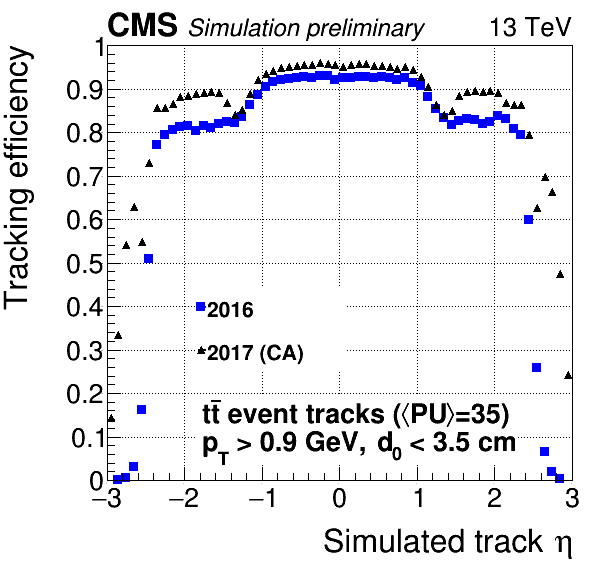
\includegraphics[width=0.95\linewidth]{Chapitre4/Images/efficiency_eta_1.png} 
    \caption*{} 
  \end{subfigure}
  \begin{subfigure}{0.5\linewidth}
    \centering
    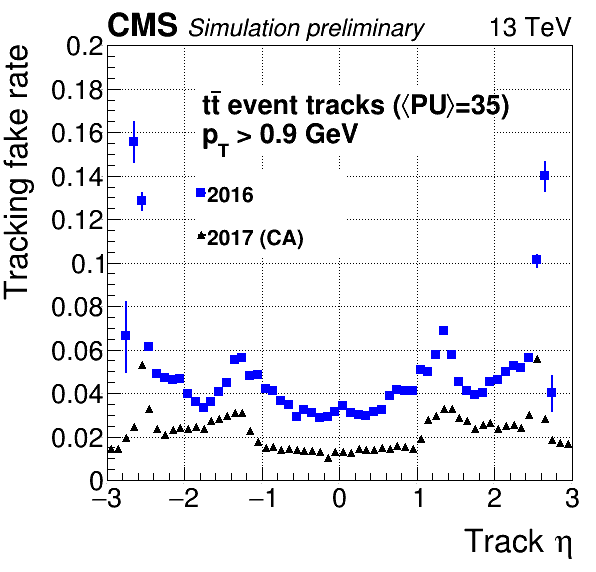
\includegraphics[width=0.95\linewidth]{Chapitre4/Images/fake_eta_1.png} 
    \caption*{} 
  \end{subfigure} 
  \caption{Efficacité de reconstruction (gauche) et taux de faux (droite) pour des traces reconstruites dans des échantillons $t\overline{t}$ simulés en fonction de la coordonnées $\eta$. Les performances avant (bleu) et après (noir) l'ajout de pixels au sein du trajectographe sont également comparées \cite{Elmetenawee:2020emw}.}
  \label{etatrackefficiency}
\end{figure}

Dans le cas des calorimètres, un algorithme de regroupement (\textit{clustering algorithm}) est utilisé afin de collecter les dépôts d'énergie et former des amas. Cet algorithme a notamment pour but de mesurer l'énergie des particules neutres dans le calorimètre électromagnétique en les isolant des particules chargées, ainsi que de regrouper les photons issus du rayonnement de freinage des électrons. Dans un premier temps l'algorithme identifie les maxima locaux d'énergie au-delà d'un certain seuil puis les associe aux cellules voisines dont l'énergie est au moins deux fois significativement supérieure au bruit (de $80$ MeV à $300$ MeV dans l'ECAL et jusqu'à 800 MeV dans le HCAL) pour former des amas dits "topologiques". \\

\begin{figure}[!ht]
\centering
    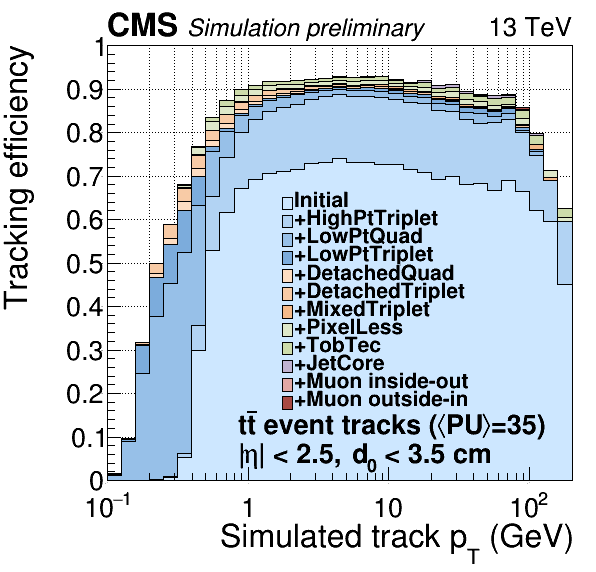
\includegraphics[width=0.55\linewidth]{Chapitre4/Images/MC_eff.png} 
    \caption{Efficacité de reconstruction pour des traces reconstruites dans des échantillons $t\overline{t}$ simulés en fonction de l'impulsion transverse. Les performances dans différentes sous parties du détecteurs et pour différents types de \textit{seed} initiale sont également présentées \cite{Elmetenawee:2020emw}.}
    \label{pttrackefficiency}
\end{figure} 

Enfin, un algorithme de raccordement (\textit{link algorithm}) est utilisé afin d'établir un lien entre traces et amas, ainsi qu'entre amas des différents calorimètres. Les traces sont d'abord propagées aux calorimètres couche par couche depuis la position de leur dernier impact dans le trajectographe, puis sont associées à un amas donné si la position de la trace et celle de l'amas coïncident dans le plan $\eta$-$\phi$. Deux amas sont ensuite associés si l'amas du calorimètre électromagnétique est englobé dans celui du calorimètre hadronique dans le plan $\eta$-$\phi$. Une procédure similaire est appliquée dans les parties avant du détecteur en considérant en plus les amas du système de \textit{preshowering} du ECAL en englobant l'amas du calorimètre le plus granulaire dans celui du moins granulaire. Finalement les éléments entre lesquels l'algorithme a établi un lien direct ou indirect sont regroupés pour former des "blocs".

\subsection{Muons}
\label{MuonID}

\begin{figure}[]
\centering
    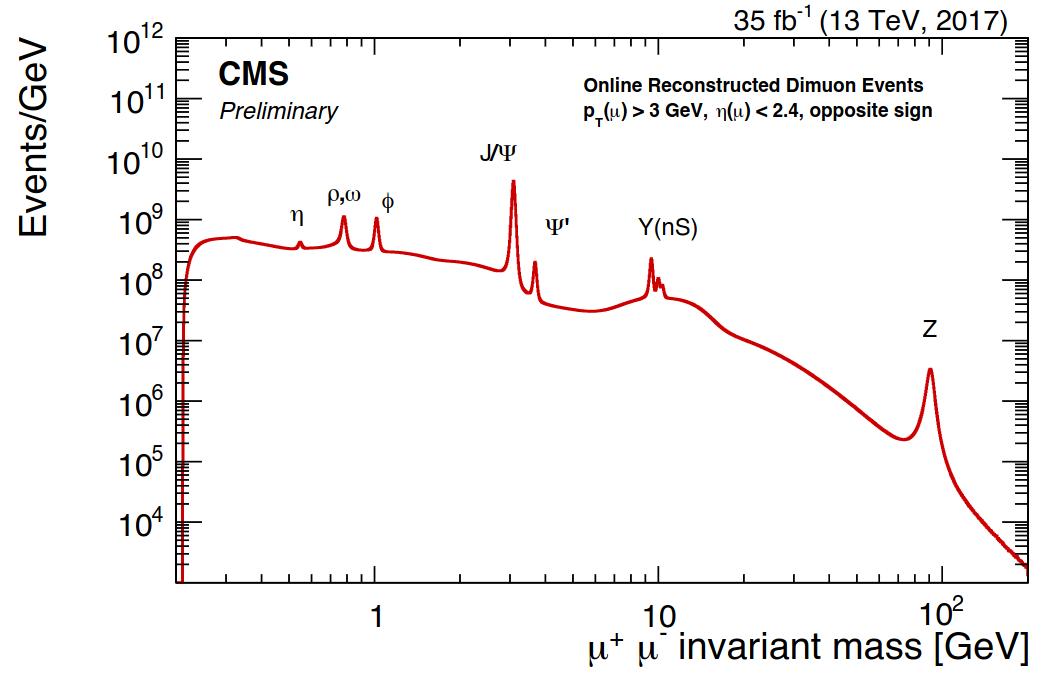
\includegraphics[width=0.8\linewidth]{Chapitre4/Images/dimuon.png} 
    \caption{Masse invariante des paires de muons $\mu^+\mu^-$ sélectionnées par le système de déclenchement et reconstruites par le détecteur CMS dans les données 2017 \cite{Dimuon}.}
    \label{dimuon}
\end{figure} 

Les muons sont les candidats les plus facilement identifiables, notamment grâce à leur capacité à traverser l'intégralité des couches du détecteur, et sont donc traités en premier par l'algorithme du flux de particules \cite{Sirunyan:2313130}. Une trace reconstruite dans le trajectographe par l'algorithme CTF sera associée à un muon (\textit{tracker muon}) dans le cas où cette dernière possède une impulsion totale supérieure à $2,5$ GeV pour une composante transverse d'au moins $0,5$ GeV et si elle coïncide avec au moins un segment des chambres à muons. La correspondance entre segment et trace est vérifiée si leur distance selon l'axe $x$ est inférieure à $3$ cm ou si le quotient de cette distance par son erreur est inférieur à 4. D'autre part une trace peut être reconstruite de manière isolée dans les chambres à muons (\textit{stand-alone muon}) par combinaison des informations des différents sous-détecteurs de ces dernières par application de filtres de Kalman. Enfin un muon dit "global" (\textit{global muon}) est reconstruit par propagation de la trace d'un \textit{stand-alone muon} à celle d'un \textit{tracker muon} si ces deux traces sont compatibles à travers un ajustement combiné et en choisissant l'association dont l'erreur est minimale si plusieurs candidats existent. Environ $99$\% des muons contenus dans l'acceptance géométrique du détecteur sont ainsi reconstruits dans le trajectographe et le plus souvent de manière globale. Les muons reconstruits par le trajectographe seul possèdent une meilleure efficacité de reconstruction dans les zones du détecteur à faible instrumentation et pour les muons à basse impulsion transverse. Ils souffrent toutefois d'une plus haute probabilité d'erreur d'identification, notamment en raison de certaines gerbes hadroniques de haute impulsion capables d'atteindre les premiers segments des chambres à muons. Les traces reconstruites dans les chambres à muons uniquement sont quant à elles sujettes à une plus grande contamination par les muons cosmiques et possèdent une plus faible résolution sur l'impulsion. La combinaison des informations du trajectographe et des chambres à muons permet alors de diminuer le taux de faux muons et d'améliorer la résolution sur leur impulsion, en particulier pour une impulsion transverse supérieure à $200$ GeV. La figure \ref{dimuon} présente une distribution de la masse invariante des paires de muons reconstruites par le détecteur CMS. L'excellente résolution permet notamment d'observer les résonances les plus connues issues de la désintégration de mésons ou du boson $Z$. \\

Par la suite, une série de variables destinées à caractériser les muons reconstruits est mise en place afin de permettre d'effectuer une sélection basée sur un équilibre entre pureté et efficacité. Ces dernières reposent notamment sur le nombres d'impacts de la trace, le nombre de segments associés ou encore la qualité de l'ajustement. D'autres peuvent également servir à différencier un muon issu du vertex primaire (\textit{prompt muon}) comme dans le cas d'une désintégration $Z\rightarrow\mu^+\mu^-$ de ceux issus d'un vertex secondaire. C'est notamment le cas de la variable relative d'isolement qui est définie comme le quotient de la somme de l'énergie des particules dans un cône $\Delta R=\sqrt{(\Delta\phi)^2+(\Delta\eta)^2}$ autour du muon et de son impulsion transverse.

\subsection{Électrons et photons isolés}
\label{EGammaID}

Plusieurs phénomènes d'interaction rayonnement-matière font de l'identification des électrons et des photons deux processus complémentaires et indissociables. D'une part, les électrons sont sujets à la perte d'une fraction de leur énergie par rayonnement de freinage au sein du trajectographe sous formes de photons. D'autre part, les photons sont susceptibles de créer des paires e$^+$/e$^-$. Dans les deux cas, électrons et photons vont de manière générale venir déposer leur énergie au sein de calorimètre électromagnétique non plus sous la forme d'une seule particule mais sous celle d'une gerbe électromagnétique. Leur reconstruction et identification est entièrement intégrée dans l'algorithme du flux de particules et s'appuie sur les traces et amas dont la construction est décrite au début de ce chapitre. Dans un premier temps, plusieurs amas du calorimètre électromagnétique sont regroupés en "superamas" (SC, \textit{superclusters}) dans une région étroite en $\eta$ et étendue en $\phi$ autour d'un amas choisi comme étant celui avec un maximum d'énergie et une énergie transverse supérieure à $1$ GeV. Cette procédure vise à regrouper les différentes particules d'une gerbe électromagnétique au sein d'un seul amas centré sur le dépôt d'énergie principal. Les traces du trajectrographe compatibles avec un SC servent ensuite de point de départ à l'algorithme GSF (\textit{Gaussian Sum-Filter}) \cite{Adam_2005} dont le but est de reconstruire la trace des électrons en modélisant l'énergie perdue sous forme de photons par une somme pondérée de distributions gaussiennes. En parallèle, la compatibilité du reste des traces est testée avec l'hypothèse de la trajectoire d'un électron et sont également injectées dans l'algorithme GSF en cas de succès. Les traces provenant d'une conversion de photon en paire e$^+$/e$^-$ sont quant à elles identifiées grâce à un algorithme dédié en recherchant notamment des vertex déplacés, et permettent de compléter la mesure du calorimètre électromagnétique seul. A ce stade toutes les traces GSF et superamas sont regroupés en blocs de flux de particules et sont encore indifférenciés entre électrons et photons. \\

Enfin, les candidats électrons sont formés à partir des blocs dans lesquels se trouve un superamas associé à au moins une trace GSF et un maximum de deux traces additionnelles. Les candidats photons sont quant à eux formés à partir des blocs dans lesquels un superamas possède une énergie transverse supérieure à $10$ GeV et sans lien établi avec une trace GSF. Les candidats issus de cette sélection forment une première collection d'électrons et de photons utilisée dans la plupart des analyses s'appuyant sur ce type d'objets. 

\subsection{Hadrons et photons non isolés}
\label{HadID}

Les hadrons constituent les derniers éléments reconstruits et identifiés par l'algorithme du flux de particules avant la reconstruction d'objets plus complexes. Ces derniers sont généralement directement reconstruits en tant que hadrons chargés ($\pi^{\pm}, K^{\pm}, p$) ou neutres ($K^0_L, n$), mais peuvent également être reconstruits sous la forme de photons non isolés dans le cas de la désintégration $\pi^0\rightarrow\gamma\gamma$ du pion neutre dont le rapport d'embranchement est de $98,823\pm0.034\%$ \cite{PDG2022}. \\

De manière générale, les photons et les hadrons neutres sont associés à des dépôts d'énergie au sein des calorimètres dont aucun lien n'a été établi avec une trace. Pour les régions du détecteur situées dans l'acceptance du trajectographe ($|\eta|<2.5$), chaque dépôt d'énergie n'ayant pas été associé à une trace dans le calorimètre électromagnétique est associé à un photon tandis qu'un dépôt dans le calorimètre hadronique est associé à un hadron neutre. Cette hypothèse repose sur le principe qu'environ $25\%$ de l'énergie des gerbes hadroniques provient de photons tandis que les hadrons neutres sont responsables de seulement $3\%$ de l'énergie déposée dans le calorimètre électromagnétique. En dehors de cette acceptance, les hadrons chargés et neutres ne sont pas différenciables et entraînent le dépôt de 25$\%$ de l'énergie des jets au sein du calorimètre électromagnétique. Les photons sont alors identifiés dans ces régions lorsqu'un amas dans le calorimètre électromagnétique n'est associé à aucun amas dans le calorimètre hadronique, puis les amas entre lesquels un lien est établi sont associés à des hadrons. Afin d'identifier les éventuels photons et hadrons neutres dont les dépôts d'énergie serait superposés à ceux de hadrons chargés, l'algorithme s'appuie sur une procédure de calibration précise des dépôts d'énergie produits par des particules neutres réalisés en amont des prises de données grâce à des tests sur faisceaux, par exposition à des sources radioactives ou encore par mesure du rayonnement cosmique. \\

Après calibration des photons et hadrons précédemment identifiés, les amas restants dans le calorimètre hadronique sont associés à une ou plusieurs traces du trajectographe, elles-mêmes ensuite associées aux éventuels amas restants dans le calorimètre électromagnétique à raison de une trace par amas. Le contenu exact des blocs ainsi formés est identifié grâce à la somme des impulsions des traces incluses. Dans le cas où la somme des impulsions est supérieure à l'énergie calibrée du bloc avec une différence supérieure à la résolution en énergie des hadrons, la présence de photons et de hadrons neutres est indiquée. Si cette différence se situe entre l'énergie déposée dans le calorimètre électromagnétique seul et une valeur maximale de $500$ MeV, un photon dont l'énergie est égale à la différence mesurée est identifié. Au-delà, un photon dont l'énergie est égale à l'énergie déposée dans le calorimètre électromagnétique seul est identifié et l'énergie restante est attribuée à la présence d'un hadron neutre lorsque celle-ci est supérieure à $1$ GeV. Enfin, chaque trace donne lieu à un hadron chargé dont les propriétés cinématiques sont celles de la trace et dont la masse est fixée à celle d'un pion chargé. Lorsque l'énergie calibrée du bloc est compatible avec la somme des impulsions des traces alors aucun hadron neutre n'est reconstruit. Dans de plus rares cas, l'énergie calibrée peut également être inférieure à la somme des impulsions des traces. Dans ce cas, une recherche de muon est effectuée, ces derniers déposant généralement peu d'énergie au sein des calorimètres. Dans $0,001\%$ des cas, si un excès est toujours observé, la recherche se porte sur la qualité de reconstruction des traces et une potentielle exclusion lorsque l'erreur associée à une trace est supérieure à $1$ GeV.

\section{Jets et énergie transverse manquante (MET)}
\label{JetMetID}

\begin{figure}
\centering
    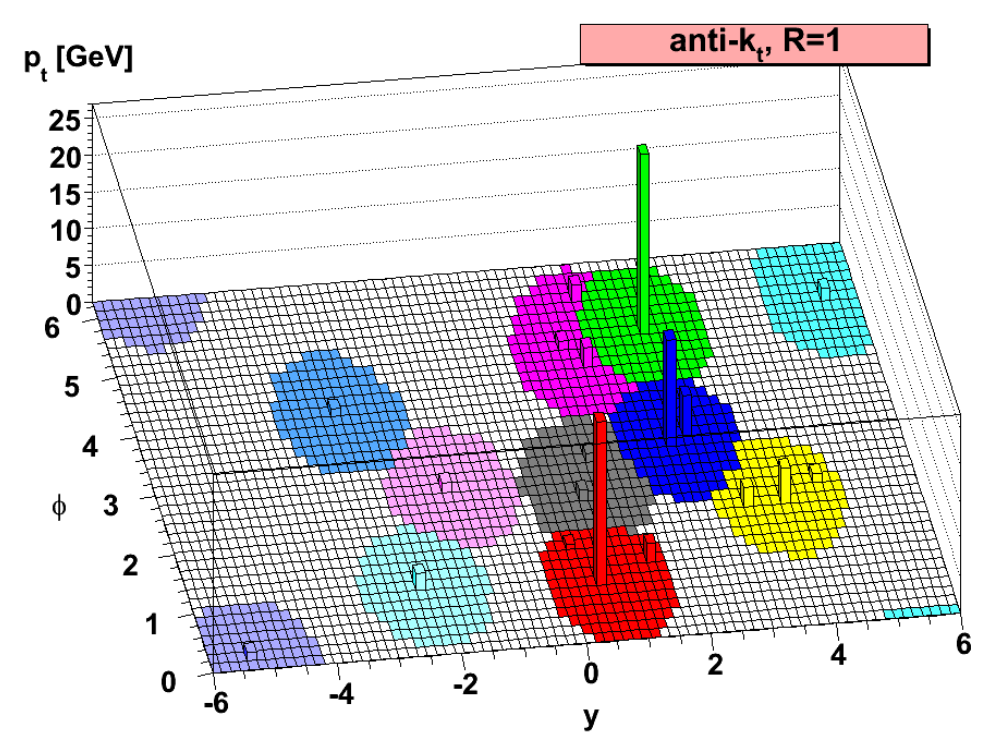
\includegraphics[width=0.55\linewidth]{Chapitre4/Images/antikt.png} 
    \caption{Représentation des jets reconstruits par l'algorithme anti-$k_t$. Chaque couleur représente un \textit{cluster} différent \cite{antikt}.}
    \label{antikt}
\end{figure} 

Une des propriétés fondamentale de la QCD est d'imposer aux quarks un confinement à travers lequel ces derniers ne peuvent exister à l'état libre tel que mentionné dans la section \ref{QCD}. Cette propriété donne lieu à un processus d'hadronisation durant lequel quarks et gluons forment des jets de hadrons au sein du détecteur. L'algorithme du flux de particules permet la reconstruction de ces objets par association des différents éléments reconstruits précédemment en s'appuyant sur un algorithme de regroupement anti-$k_t$ (\textit{anti-$k_t$ jet clustering algorithm}) \cite{antikt}, où $k_t$ désigne l'impulsion transverse ($p_T$) d'un objet. Tout algorithme de regroupement s'appuie sur une définition particulière de la distance entre deux objets ($d_{ij}$) et de celle entre un objet et le faisceau ($d_iB$) en considérant tous les objets à l'intérieur d'un cône de taille donnée. Ces distances s'écrivent :

\begin{align}
    d_{ij} & = \mbox{min}\bigl(k_{ti}^{2p},k_{tj}^{2p}\bigr)\frac{\Delta_{ij}^2}{R^2}, \\
    d_{iB} & = k_{ij}^{2p},
\end{align}

avec $\Delta^2_{ij}=(y_i-y_j)^2+(\phi_i-\phi_j)^2$, et où $k_{ti}$ représente l'impulsion transverse de l'objet $i$, $y_i$ sa rapidité et $\phi_i$ sa coordonnée azimuthale. $R$ représente la taille du cône à l'intérieur duquel l'algorithme opère, fixée à $0,4$ lors du Run 2. La particularité de l'algorithme anti-$k_t$ repose sur la valeur du paramètre $p$ fixée à $-1$, où cette valeur sera positive pour un algorithme classique de type $k_t$. L'algorithme procède ensuite de manière itérative sur toutes les particules de l'évènement en calculant pour chacune les distances $d_{ij}$ et $d_{iB}$ puis en classant ces distances par ordre décroissant. En commençant par la valeur minimale, si cette distance est de type $d_{ij}$ les impulsions des particules $i$ et $j$ sont sommées. Si la distance est de type $d_{iB}$, la particule $i$ est associée à un jet puis retirée de la liste. L'algorithme répète ensuite cette procédure jusqu'à ce que tous les objets soient associés à un jet. Lorsque qu'un jet est isolé il possède une forme caractéristique conique telle que montrée dans la figure \ref{antikt}, et sa composition typique en énergie est donnée dans la figure \ref{JetEnergy}. \\

\begin{figure}[]
    \begin{subfigure}{0.5\linewidth}
    \centering
    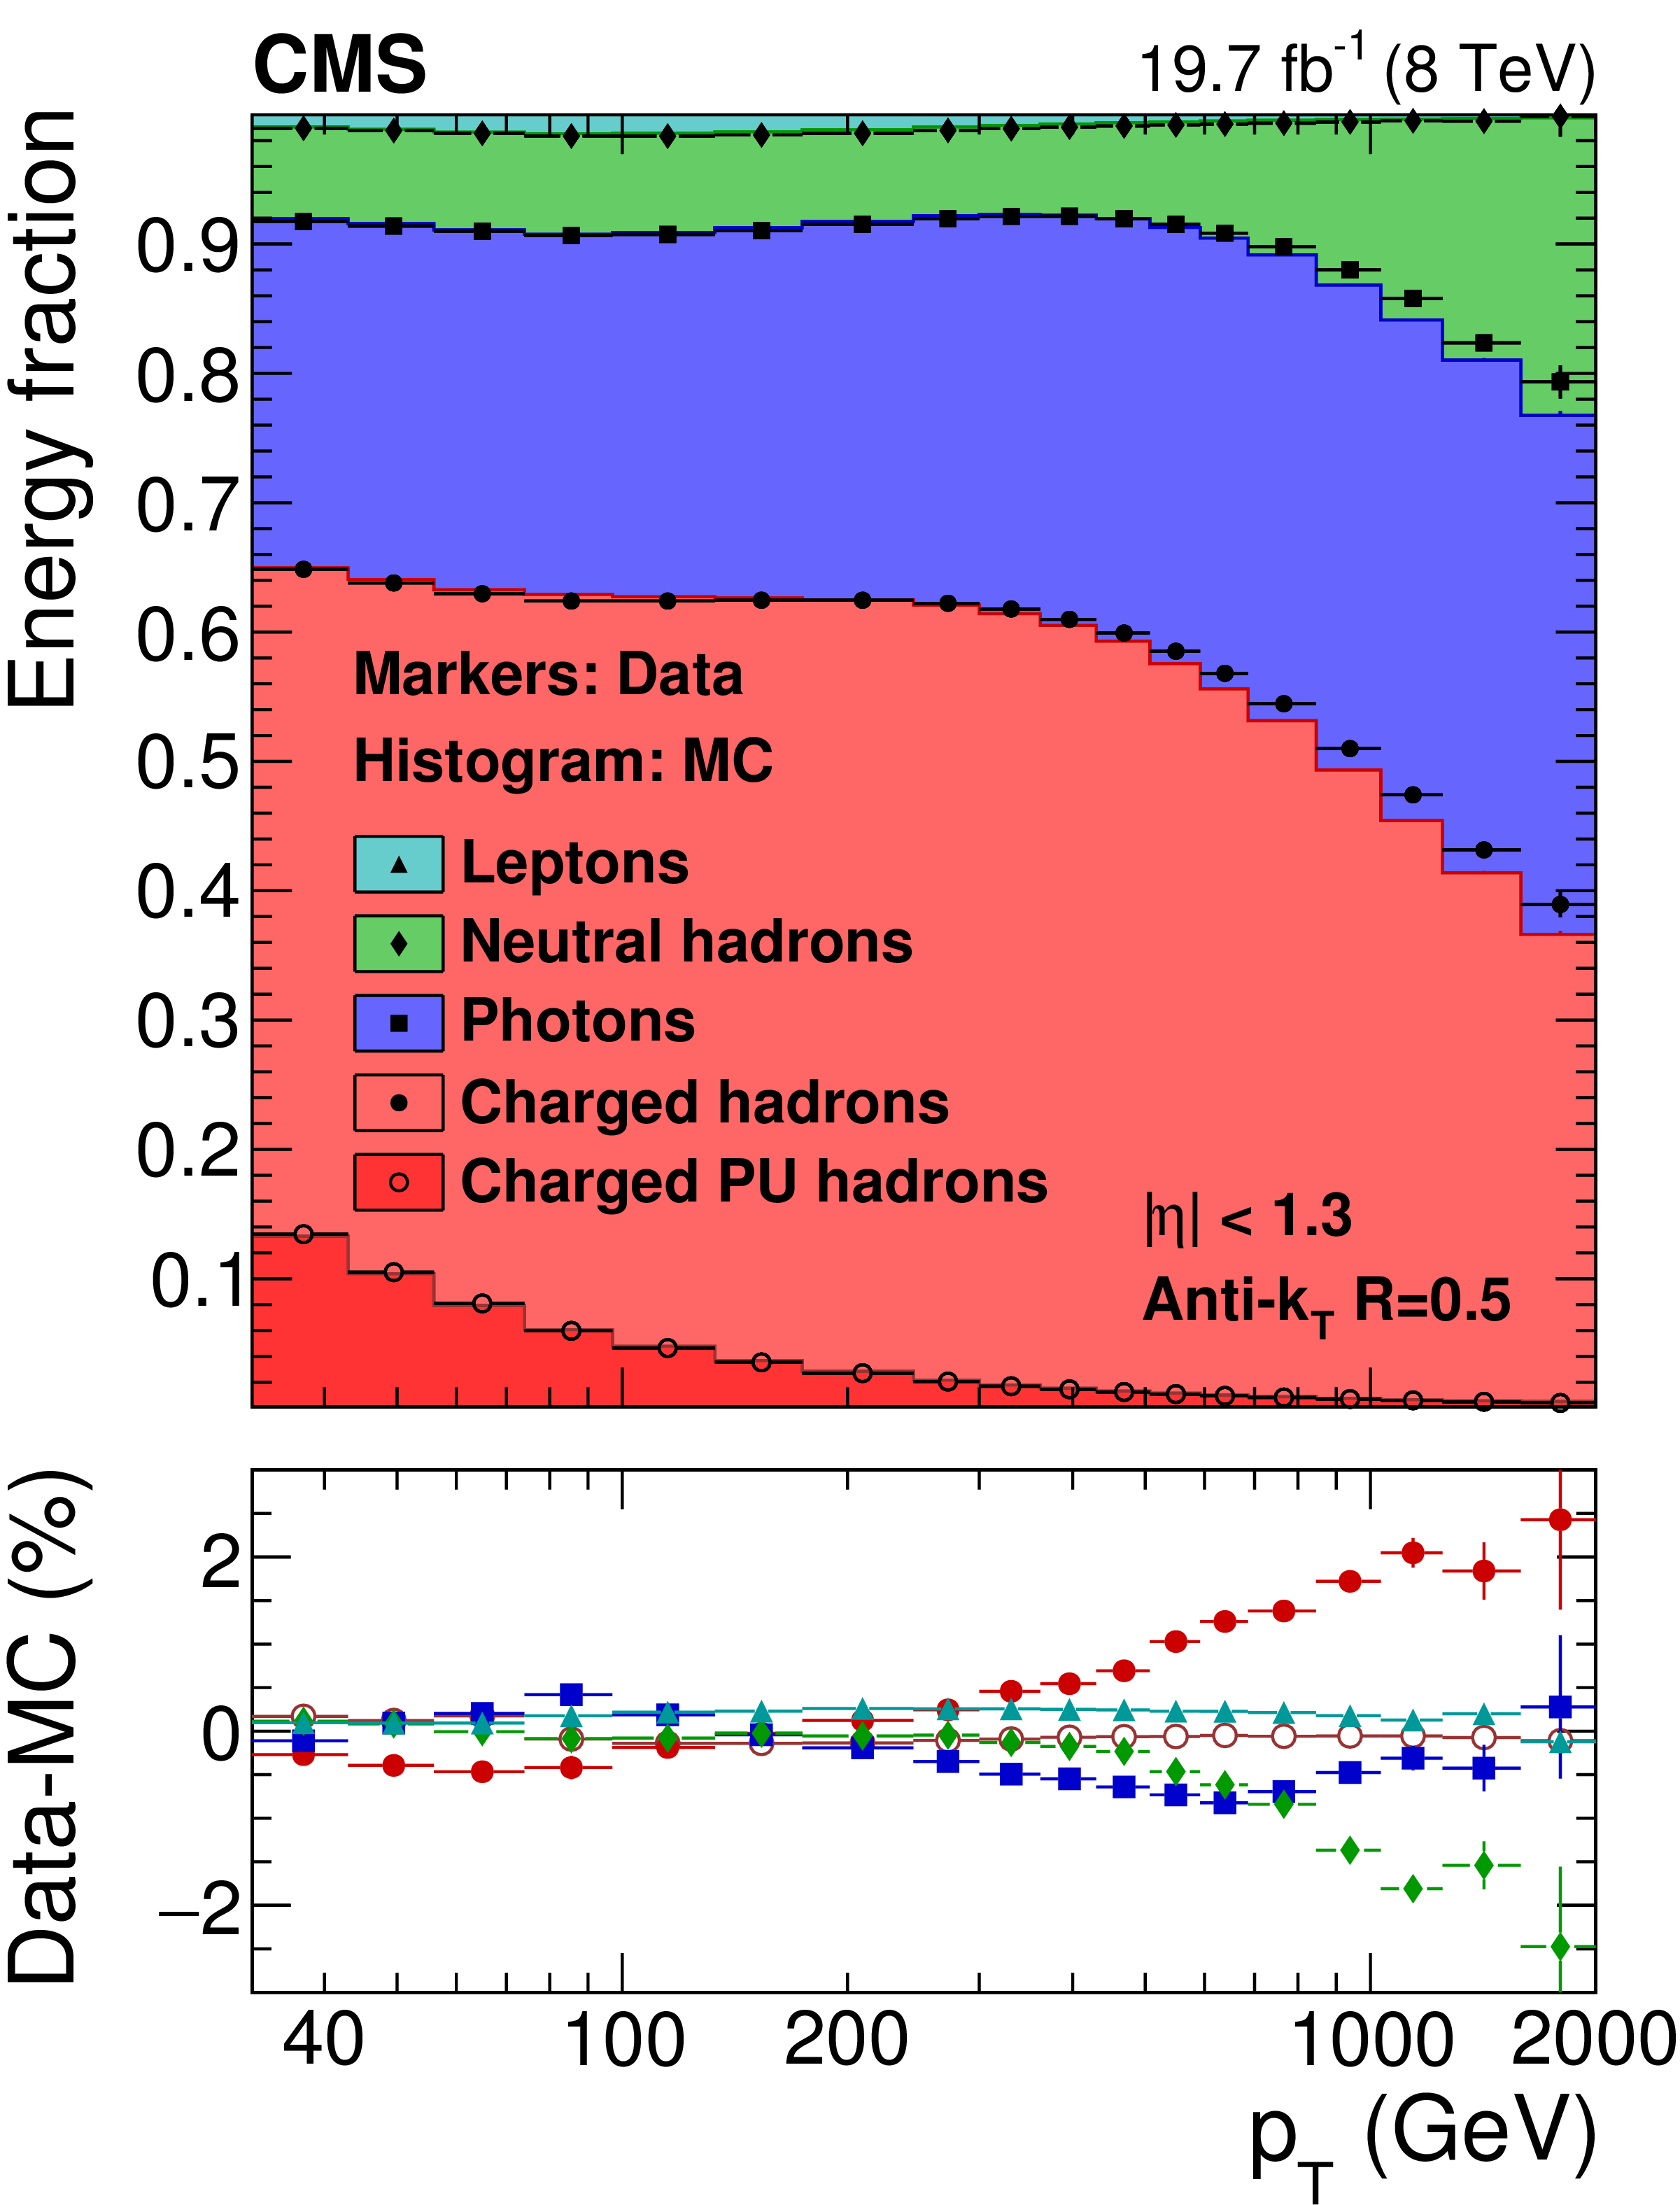
\includegraphics[width=0.95\linewidth]{Chapitre4/Images/PFJetPT.png} 
    \caption*{} 
    \end{subfigure}
    \begin{subfigure}{0.5\linewidth}
    \centering
    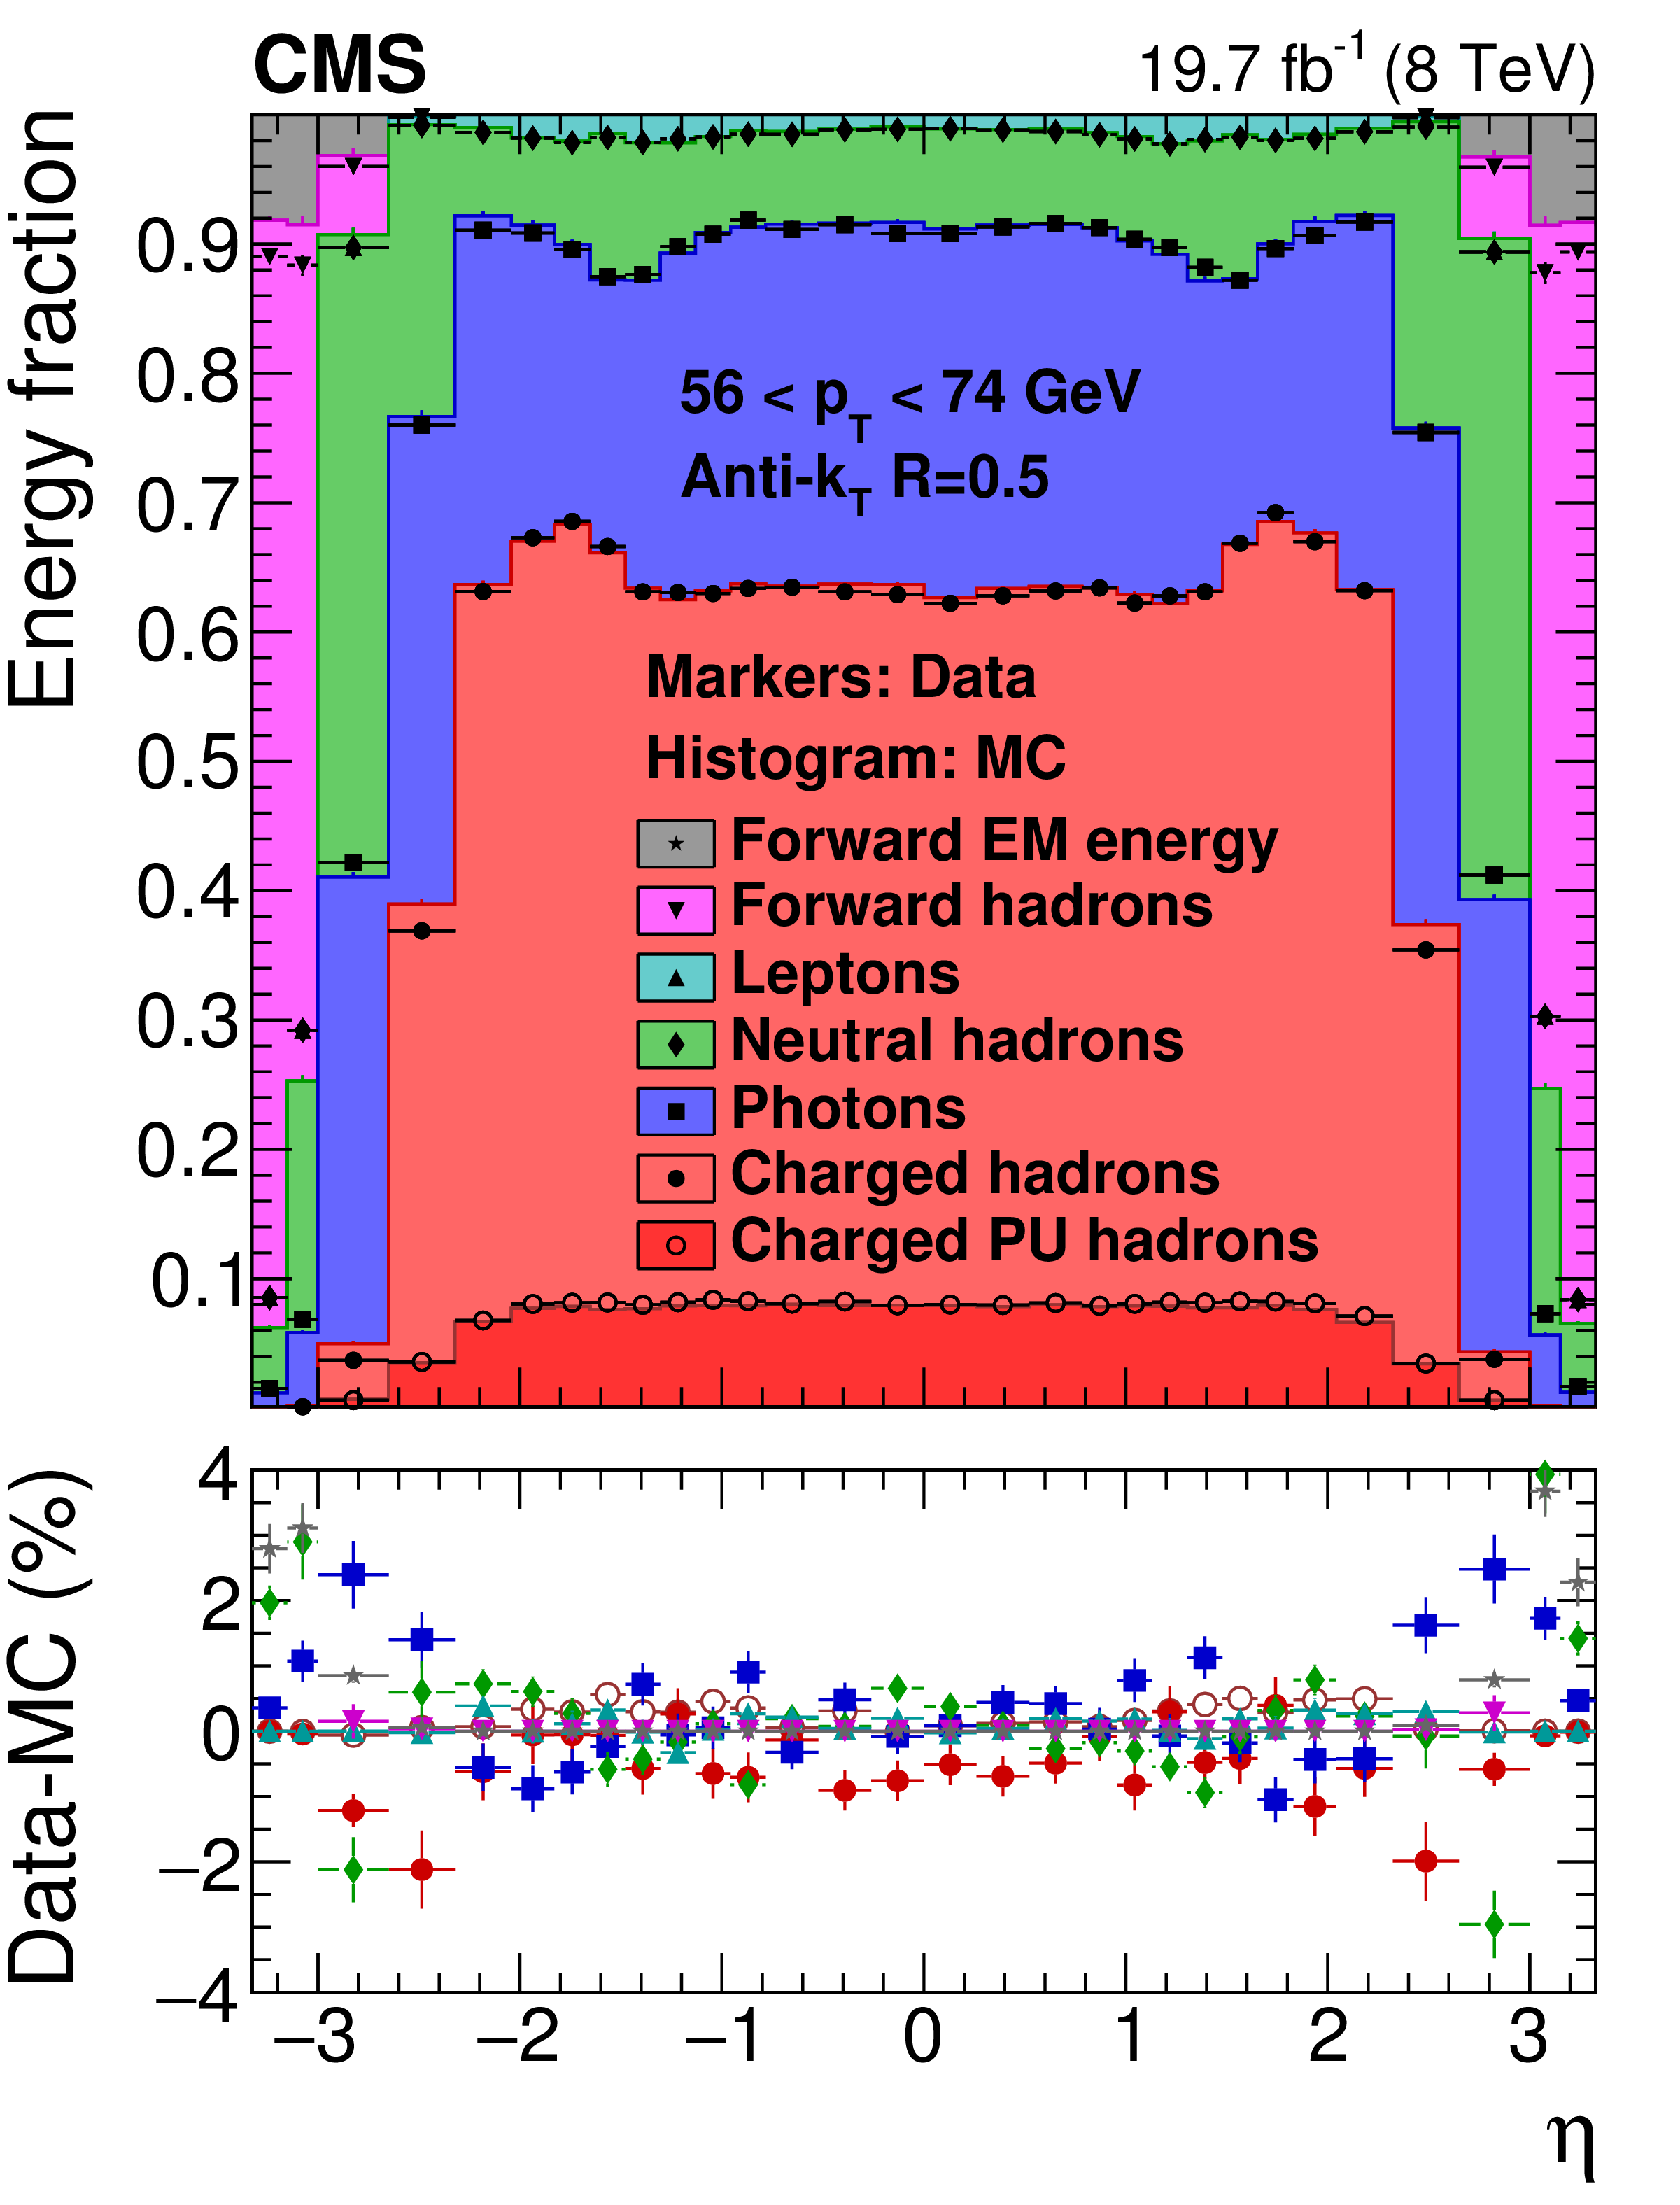
\includegraphics[width=0.95\linewidth]{Chapitre4/Images/PFJetETA.png} 
    \caption*{} 
    \end{subfigure}
    \caption{Composition en énergie des jets et comparaison entre données et simulation en fonction de l'impulsion transverse (gauche) et de la coordonnée $\eta$ (droite). Les hadrons chargés associés à un vertex issu de l'empilement sont dénotés "\textit{Charged PU hadrons}" \cite{ThePFAlgo}.}
    \label{JetEnergy}
\end{figure}

La MET peut être déterminée à partir de l'inverse de la somme des impulsions transverses de tous les objets directement issus de l'algorithme du flux de particules au sein d'un évènement et est alors appelée PF MET. Elle peut également être mesurée à partir des informations des calorimètres seuls (Calo MET). Une comparaison de la résolution entre cette dernière et la PF MET est donnée dans la figure \ref{METreso}. Enfin, l'algorithme PUPPI \cite{puppi} sera également introduit dans la section \ref{MET} pour les besoins de l'analyse présentée dans le chapitre \ref{analysis}.

\begin{figure}
    \centering
    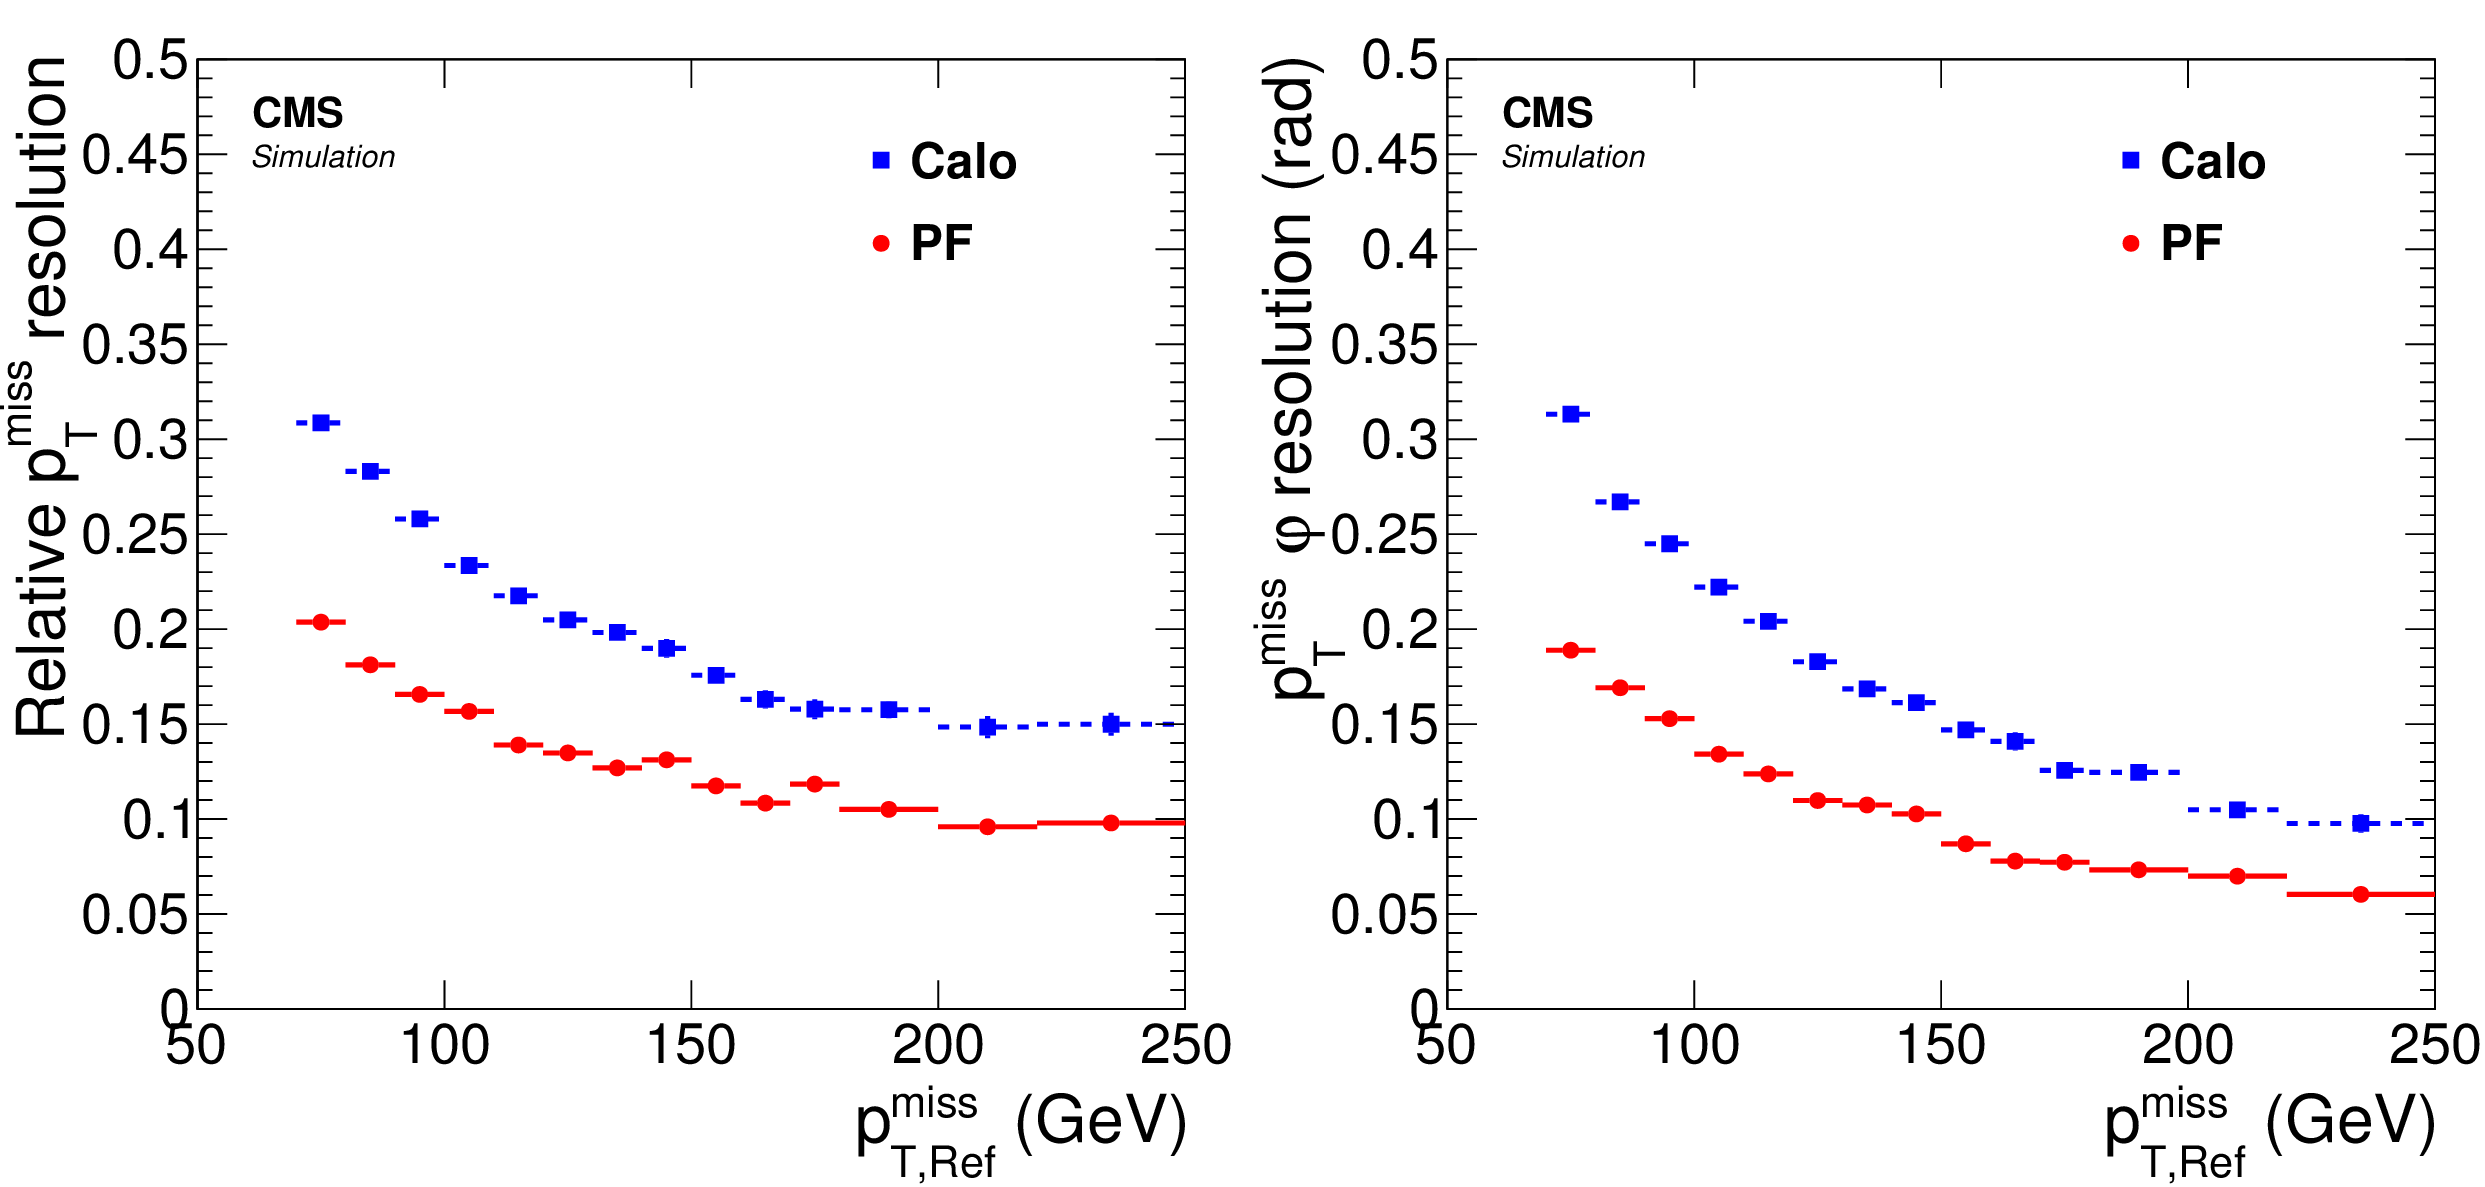
\includegraphics[scale=0.15]{Chapitre4/Images/METres.png}
    \caption{Résolution relative et résolution angulaire de la PF MET et de la Calo MET mesurées dans des échantillons d'évènements $t\overline{t}$ simulés \cite{ThePFAlgo}.}
    \label{METreso}
\end{figure}

\section{Leptons tau}

Ce paragraphe vise à introduire les propriétés du lepton tau ainsi que les méthodes de reconstruction et d'identification employées au sein de CMS. D'autres méthodes, propres aux besoins de l'analyse de la structure CP du couplage de Yukawa du lepton tau, seront également présentées dans la section \ref{eventreco} du chapitre \ref{analysis}.

\begin{figure}[b]
\centering
    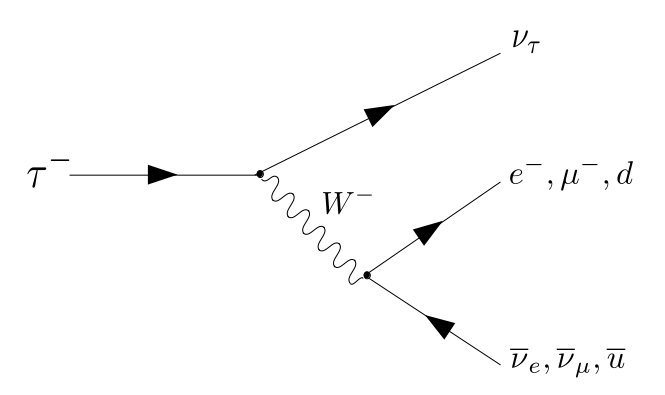
\includegraphics[width=0.6\linewidth]{Chapitre4/Images/taudecay.png} 
    \caption{Diagramme de Feynman associé à la désintégration d'un lepton tau.}
    \label{taudecay}
\end{figure} 

\subsection{Propriétés}
\label{tau properties}
Le lepton tau appartient à la troisième génération des fermions avec une masse $m_{\tau}=1.77$ GeV$\simeq3500~m_e$ faisant de lui une particule hautement instable. Sa désintégration fait intervenir un courant chargé (fig. \ref{taudecay}) à travers lequel un neutrino tau est produit. Le boson W intermédiaire produit dans un tiers des cas une désintégration leptonique vers un électron ou un muon accompagné d'un neutrino de même saveur, et une désintégration hadronique à travers une paire de quark dans les deux tiers des cas restants. Les différents états finaux de la désintégration du lepton tau et leur rapport d'embranchement sont présentés dans le tableau \ref{tabDM}. Son temps de vie de l'ordre de $10^{-13}$ secondes lui offre un temps de vol trop court pour atteindre les premières couches de détection du trajectographe de CMS et ainsi seuls ses produits de désintégration, à l'exception des neutrinos, sont détectés. \\

\begin{table}[h]
\centering
\begin{tabular}{|ll|l|ll}
\hline \hline
\multicolumn{2}{c|}{\begin{tabular}[c]{@{}c@{}}Mode de désintégration\\ $\tau^-\rightarrow$\end{tabular}}                                          & \multicolumn{1}{c|}{\begin{tabular}[c]{@{}c@{}}Résonance\\ intermédiaire\end{tabular}} & \multicolumn{2}{c}{BR(\%)}                       \\ \hline \hline
\multicolumn{1}{c|}{\multirow{2}{*}{Leptonique}} & e$^-\overline{\nu}_e\nu_{\tau}$   &                                                                                        & \multicolumn{1}{l|}{17.4} & \multirow{2}{*}{35.2} \\[3pt] \cline{2-4}
\multicolumn{1}{c|}{}                            & $\mu^-\overline{\nu}_e\nu_{\tau}$ &                                                                                        & \multicolumn{1}{l|}{17.8} &                       \\ [3pt] \hline \hline
\multicolumn{1}{l|}{\multirow{6}{*}{Hadronique}} & $\pi^-\nu_{\tau}$                 &                                                                                        & \multicolumn{1}{l|}{11.5} & \multirow{6}{*}{64.8} \\ [3pt]\cline{2-4}
\multicolumn{1}{l|}{}                            & $\pi^-\pi^0\nu_{\tau}$            & $\rho (770)$                                                                           & \multicolumn{1}{l|}{26.0} &                       \\ [5pt]\cline{2-4}
\multicolumn{1}{l|}{}                            & $\pi^-\pi^0\pi^0\nu_{\tau}$       & $a_1^{1pr} (1260)$                                                                     & \multicolumn{1}{l|}{9.5}  &                       \\ [3pt] \cline{2-4}
\multicolumn{1}{l|}{}                            & $\pi^-\pi^+\pi^-\nu_{\tau}$       & $a_1^{3pr} (1260)$                                                                     & \multicolumn{1}{l|}{9.8}  &                       \\ [3pt] \cline{2-4}
\multicolumn{1}{l|}{}                            & $\pi^-\pi^+\pi^-\pi^0\nu_{\tau}$  &                                                                                        & \multicolumn{1}{l|}{4.8}  &                       \\[3pt] \cline{2-4}
\multicolumn{1}{l|}{}                            & Autres                            &                                                                                        & \multicolumn{1}{l|}{3.2}  &                       \\[3pt] \hline \hline
\end{tabular}
\caption{Modes de désintégration du lepton tau et rapport d'embranchement (BR) correspondant. Dans le cas où elle existe, la résonance intermédiaire et sa masse sont également précisées.}
\label{tabDM}
\end{table}

\subsection{Reconstruction et identification}
\label{TauID}

Le court temps de vie du lepton tau ne permet que difficilement aux énergie du LHC de différencier un lepton issu d'une désintégration leptonique du tau d'un lepton issu du vertex primaire. Ainsi un muon ou un électron provenant d'un lepton tau sera reconstruit et identifié avec les mêmes méthodes présentées dans les sections \ref{MuonID} et \ref{EGammaID} respectivement. Dans le cas des désintégrations hadroniques, chaque hadron chargé produit sera identifié et reconstruit selon les méthodes présentées dans la section \ref{HadID} et serviront de point de départ à l'algorithme HPS (\textit{Hadron-Plus-Strip}) en charge de l'identification des modes de désintégration du lepton tau. L'algorithme HPS est déclenché par le hadron chargé de plus haute impulsion transverse au sein d'un jet. L'impulsion transverse d'un cône $p_T^{0.4}$ est ensuite définie comme la somme de toutes les particules au sein d'un cône $\Delta R_1 = 0.4$ centré sur la trace de plus haute impulsion transverse, avec une condition nécessaire $d_z<0.4$ cm entre la trace initiale et les autres traces associées à des hadrons chargés. Un cône de signal restreint est ensuite défini au sein du premier tel que $\Delta R_{sig} = \sfrac{2.8}{p_T^{0.4}}$ et $0.05\leq\Delta R_{sig}\leq 0.1$. L'impulsion transverse du tau hadronique est ensuite calculée comme la somme des impulsions transverses des hadrons chargés au sein du cône de signal et de celles des éventuels électrons et photons issus de la désintégration de hadrons neutres situés dans des bandes (\textit{strips}) centrées sur la trace initiale dans le plan $\eta$-$\phi$. La taille de ces bandes était de $0.05\times0.2$ lors de la première phase d'exploitation du LHC puis est devenue variable lors de la seconde afin de tenir compte de l'impulsion transverse des électrons et photons. Parmi les candidats situés en dehors des bandes déjà construites selon le premier critère, celui de plus haute impulsion transverse est choisi pour définir une nouvelle bande puis le candidat de plus haute impulsion transverse suivant est ajouté à la bande s'il se trouve dans l'intervalle :

\begin{align*}
    \Delta\eta & = f(p_T^{e/\gamma}) + f(p_T^{strip}),\; 0.05\leq\Delta\eta\leq0.15, \\
    \Delta\phi & = g(p_T^{e/\gamma}) + g(p_T^{strip}),\; 0.05\leq\Delta\phi\leq0.3,
    \vspace{5pt} 
\end{align*}

où $p_T^{e/\gamma}$ est l'impulsion transverse du candidat suivant, $p_T^{strip}$ l'impulsion transverse initiale de la bande et où $f(p_T)$ et $g(p_T)$ sont des fonctions définies par :

\begin{align*}
    f(p_T) & = 0.20 p_T^{-0.66}, \\
    g(p_T) & = 0.35 p_T^{-0.71}.
    \vspace{5pt} 
\end{align*}

La nouvelle impulsion de la bande est alors calculée comme la somme pondérée des impulsions transverses des électrons et photons à l'intérieur de celle-ci puis l'algorithme s'arrête lorsque plus aucun candidat s'inscrivant dans la fenêtre ($\eta,\phi$) de la bande n'est trouvé. A partir du nombre de hadrons chargés et de bandes au sein du cône de signal, un mode de désintégration (HPS-DM) est ensuite attribué au tau hadronique par l'algorithme HPS selon la numérotation suivante :

\begin{itemize}
    \medskip
    \item[$\bullet$] $0$ : un hadron chargé seul ($\tau_h\rightarrow h^{\pm}$),
    \medskip
    \item[$\bullet$] $1$ : un hadron chargé et une bande ($\tau_h\rightarrow h^{\pm}+\pi^0$),
    \medskip
    \item[$\bullet$] $2$ : un hadron chargé et deux bandes ($\tau_h\rightarrow h^{\pm}+2\pi^0$),
    \medskip
    \item[$\bullet$] $10$ : trois hadrons chargés ($\tau_h\rightarrow 2h^{\pm}+h^{\mp}$),
    \medskip
    \item[$\bullet$] $11$ : trois hadrons chargés et une bande ($\tau_h\rightarrow 2h^{\pm}+h^{\mp}+\pi^0$).
    \medskip
\end{itemize}

Une coupure supplémentaire sur la masse du tau hadronique peut être appliquée en fonction du mode de désintégration et de la masse de la résonance intermédiaire (table \ref{tabDM}) en jeu. \\

Par ailleurs, le jet de hadrons issu de la désintégration d'un tau hadronique peut s'apparenter à un jet issu de la QCD et mener à une erreur d'identification de celui-ci. Le taux de faux jets, notés $jet\rightarrow\tau_h$, peut toutefois être réduit par une coupure sur la variable d'isolement $I_{\tau_h}$ du lepton tau définie par :

\begin{equation*}
    I_{\tau_h}=\sum p_T^{\text{charged}}\bigl(d_z<0,2~\mbox{cm})+\max(0,\sum p_T^{\gamma}-\Delta\beta\sum p_T^{\text{charged}}(d_z>0,2~\mbox{cm})\bigr),
\end{equation*}

où $\sum p_T^{\text{charged}}$ et $\sum p_T^{\gamma}$ représente la somme scalaire de l'impulsion transverse des particules chargées et des photons PF respectivement, situés à l'extérieur du cône de signal du lepton tau et à l'intérieur d'un cône d'isolement de taille variable. Le premier terme ne tient compte que des particules pour lesquelles $d_z<0,2$ cm et à l'intérieur d'un cône d'isolement défini par $\Delta R=0,5$ afin d'exclure les contributions des particules chargées issues de l'empilement. Dans le second terme, la contribution des particules chargées pour lesquelles $d_z>0,2$ situées dans un cône de taille $\Delta R=0,8$ est soustraite à l'impulsion des photons reconstruits dans cône de taille $\Delta R=0,5$. Le facteur $\Delta\beta=0,2$ tient compte de la fraction moyenne de hadrons neutres au sein des jets de hadrons et de la taille variable du cône dans lequel la contribution de l'empilement est estimée. Trois niveaux de coupure sont définis avec $I_{\tau_h}=2,5$ GeV (\textit{Loose}), $I_{\tau_h}=1,5$ GeV (\textit{Medium}) et $I_{\tau_h}=0,8$ GeV (\textit{Tight}). Afin de limiter la mauvaise identification des leptons tau pour lesquels un photon réellement issu de la désintégration se situe en dehors du cône de signal, une seconde variable d'isolation $p_T^{\text{strip,outer}}$ est employée \cite{taureco}. Celle-ci est définie par :

\begin{equation}
    p_T^{\text{strip,outer}}=\sum p_T^{e/\gamma}(\Delta R>\Delta R_{\text{sig}}),     
\end{equation}

\vskip 0.1cm

et correspond à la somme scalaire de l'impulsion transverse des électrons et photons au sein des bandes calorimétriques identifiées par HPS mais situés en dehors du cône de signal. Un tau hadronique est alors conservé si cette quantité est inférieure à $10\%$ de son impulsion transverse. \\

Les électrons et les muons sont également sujets à une mauvaise identification en tau hadronique. L'électron génère notamment un rayonnement de freinage dont la signature expérimentale peut s'apparenter à celle d'un pion neutre dans le calorimètre électromagnétique. Un muon isolé est quant à lui susceptible d'être assimilé à un tau hadronique lorsque sa position reconstruite dans les chambres à muons est proche de celle du lepton tau dans le plan $(\eta,\phi)$. Le réseau de neurone \textit{DeepTau} \cite{deeptau} est alors employé pour l'identification des leptons tau hadroniques. Cet algorithme s'appuie sur la densité d'énergie moyenne déposée au sein d'un l'évènement ainsi que sur une série de variables cinématiques, de qualité des traces reconstruites et les dépôts d'énergie au sein des calorimètres afin de fournir 3 discriminants contre la mauvaise identification des jets, des électrons et des muons. La figure \ref{deeptauperf} présente les performances d'identification de cet algorithme ainsi qu'une comparaison aux méthodes d'identification classiques de CMS.

\begin{figure}
    \begin{subfigure}[b]{\linewidth}
    \centering
        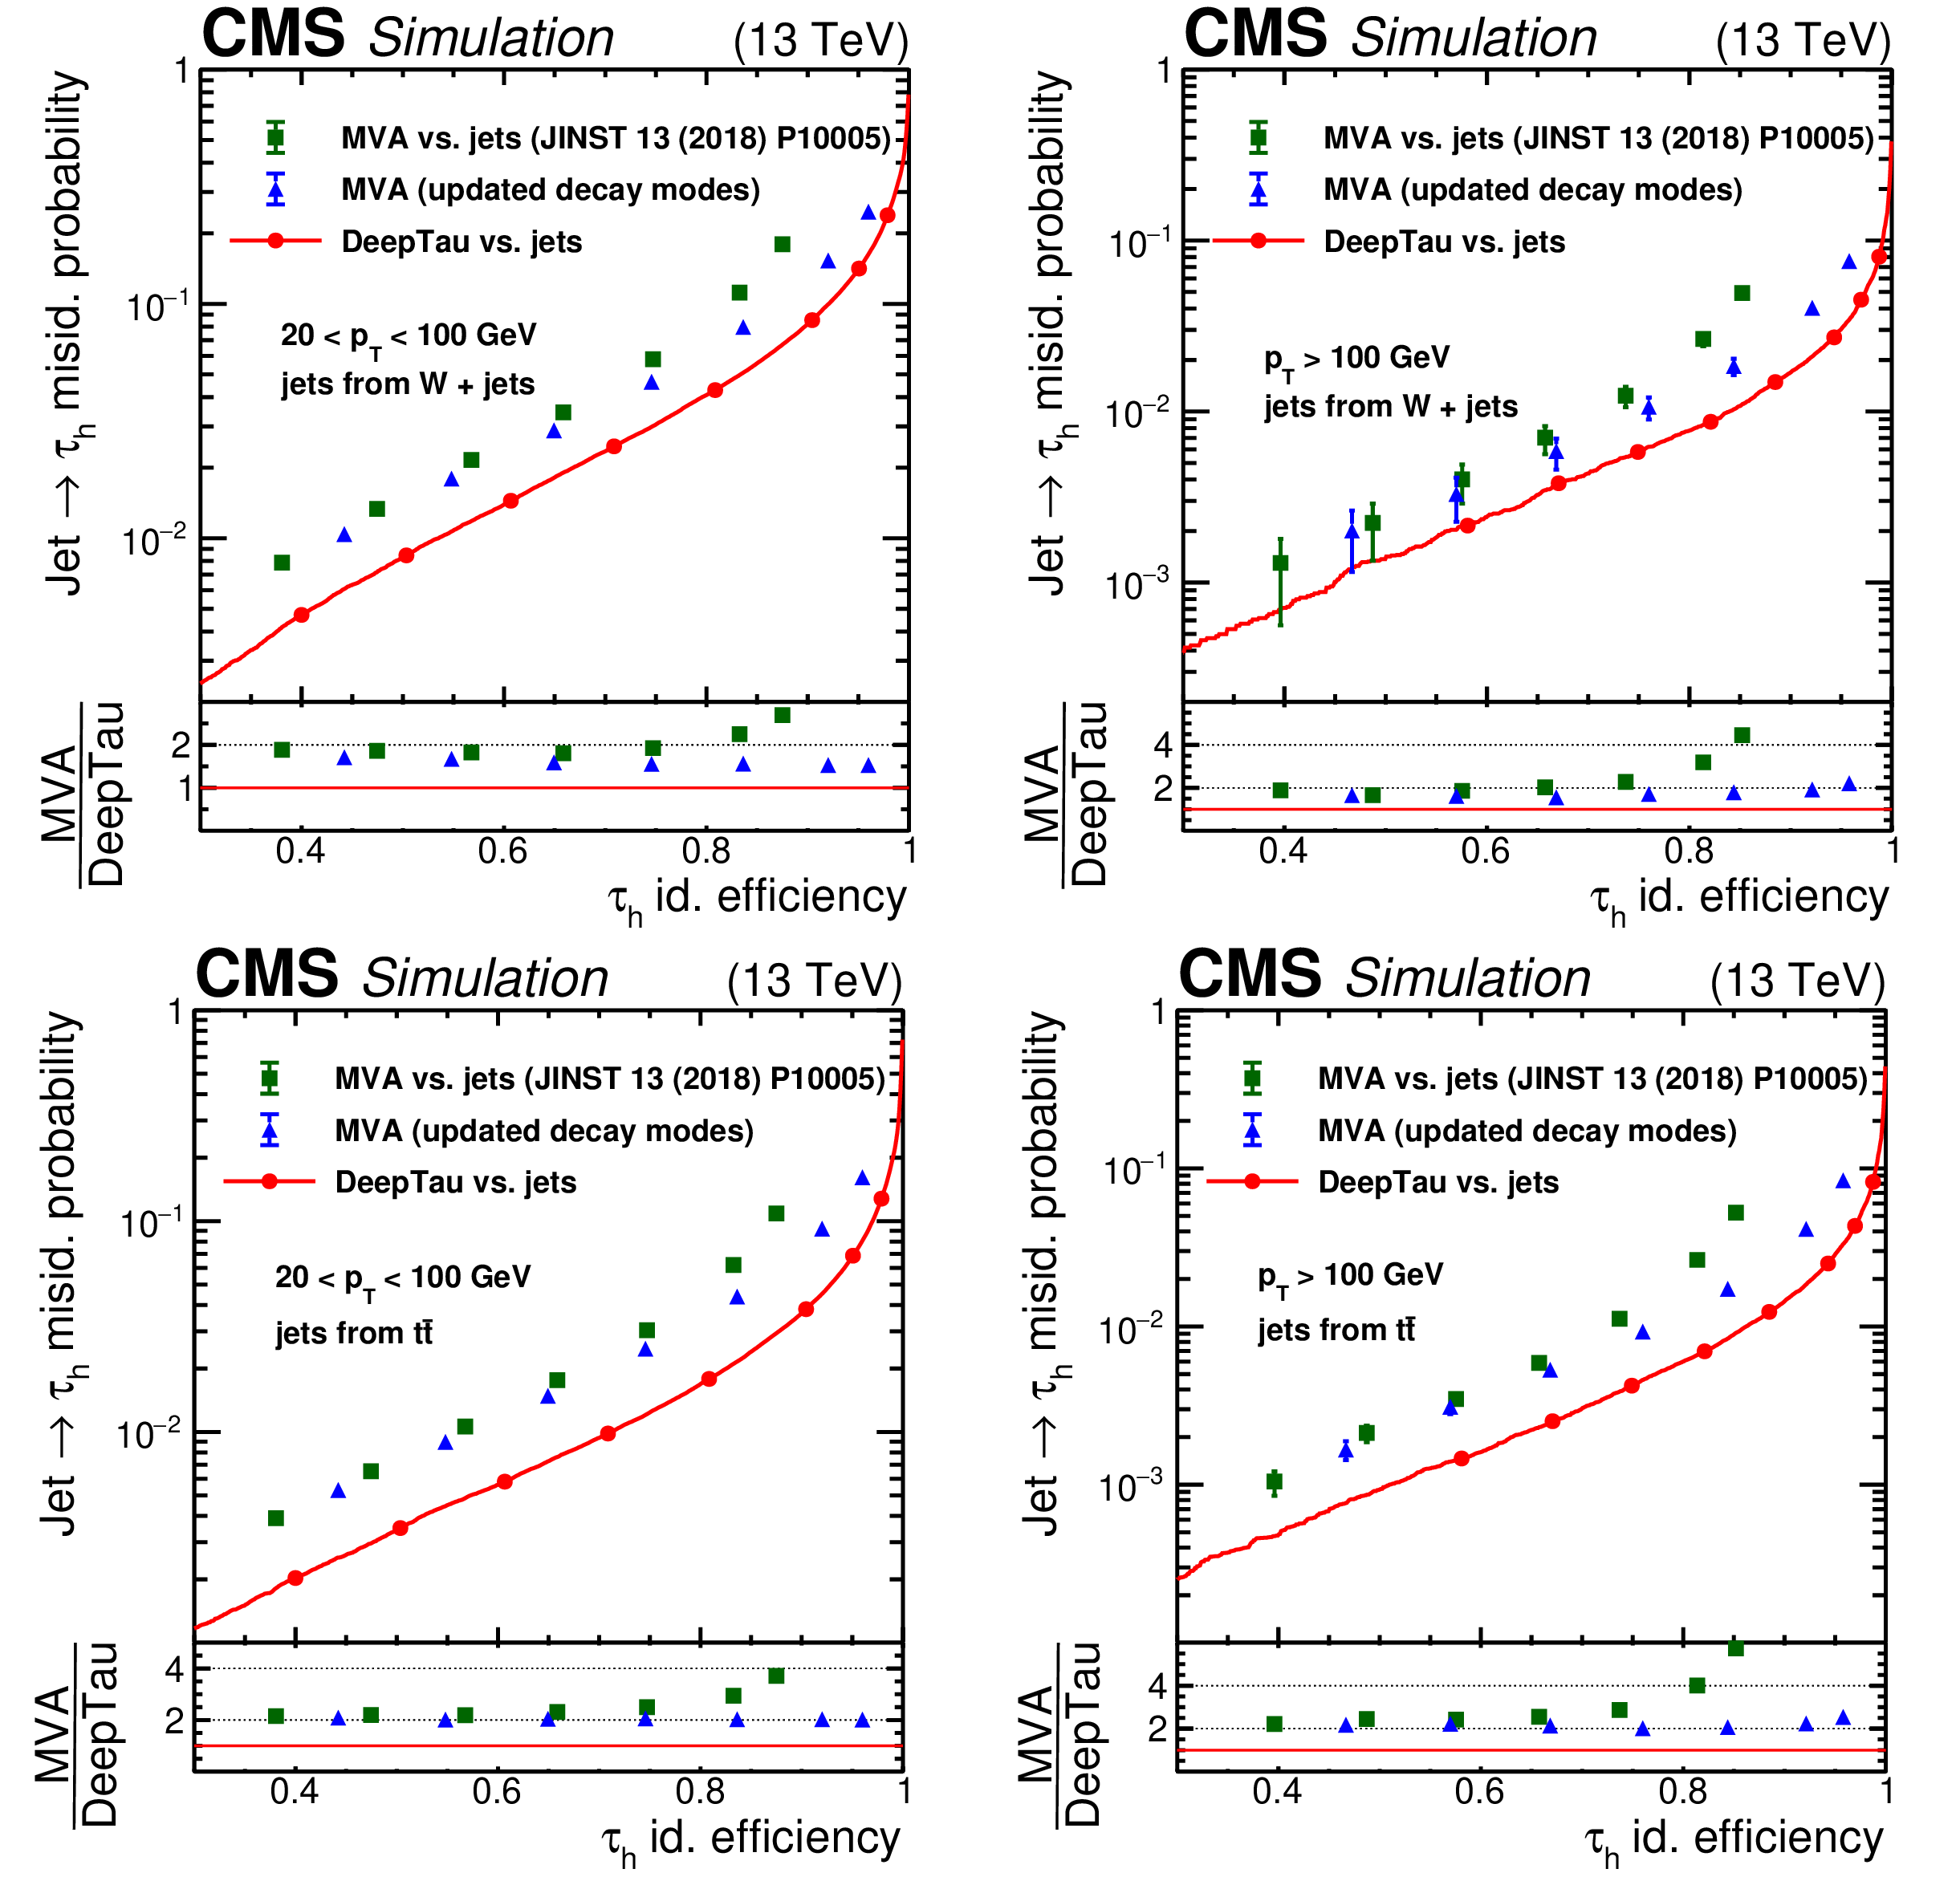
\includegraphics[scale=0.13]{Chapitre4/Images/DeepTauvsJets.png}
        \caption{}
    \end{subfigure}
    \begin{subfigure}[b]{\linewidth}
    \centering
        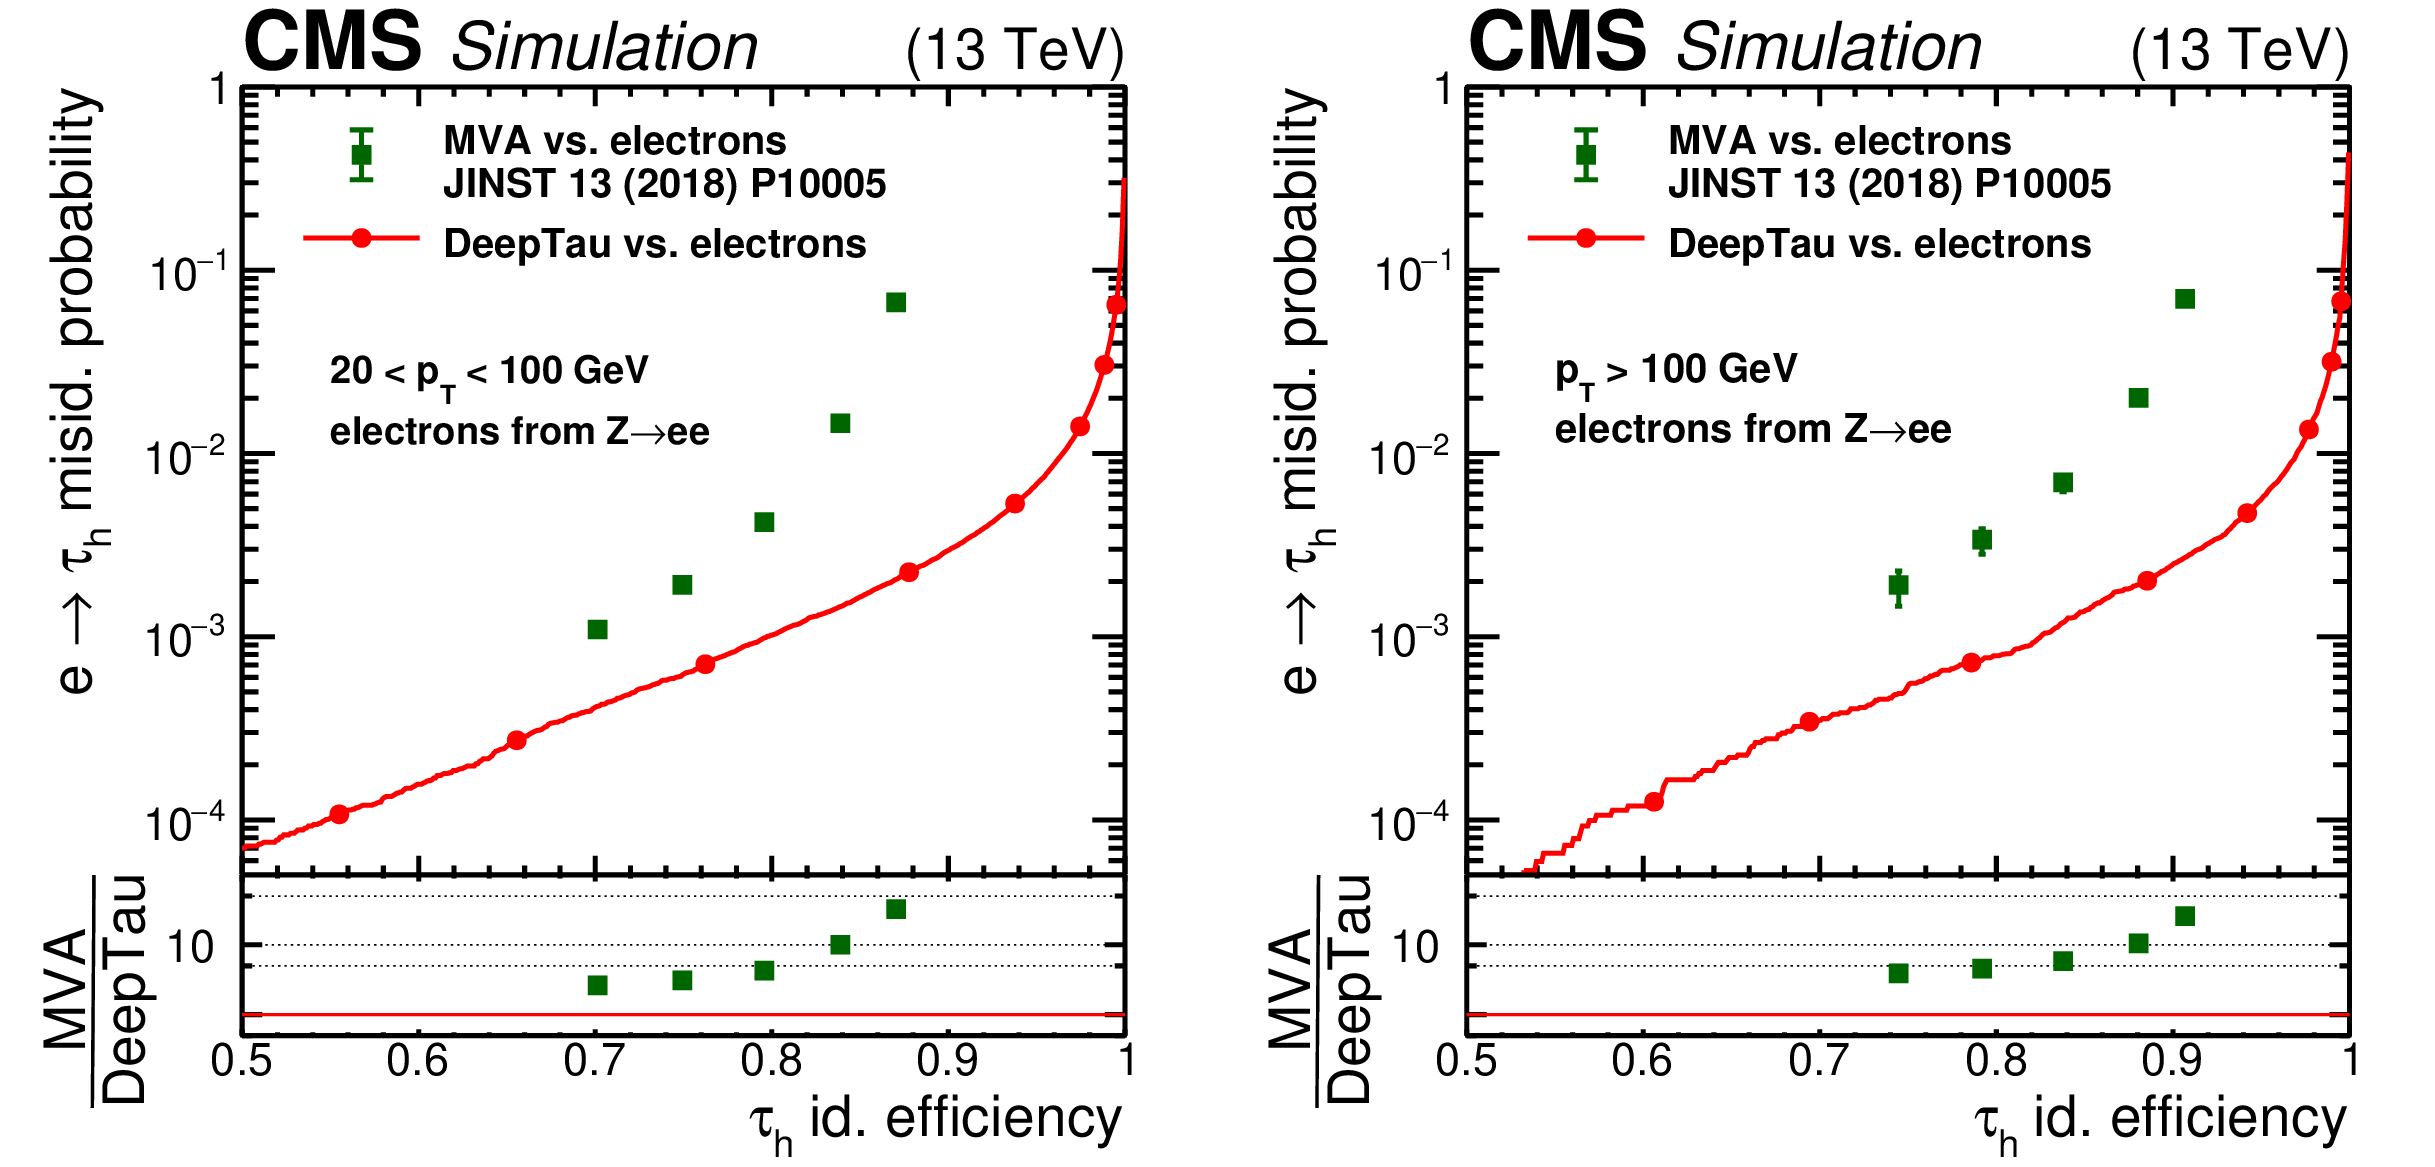
\includegraphics[scale=0.13]{Chapitre4/Images/DeepTauvsEle.png}
        \caption{}
    \end{subfigure}
    \begin{subfigure}[b]{\linewidth}
    \centering
        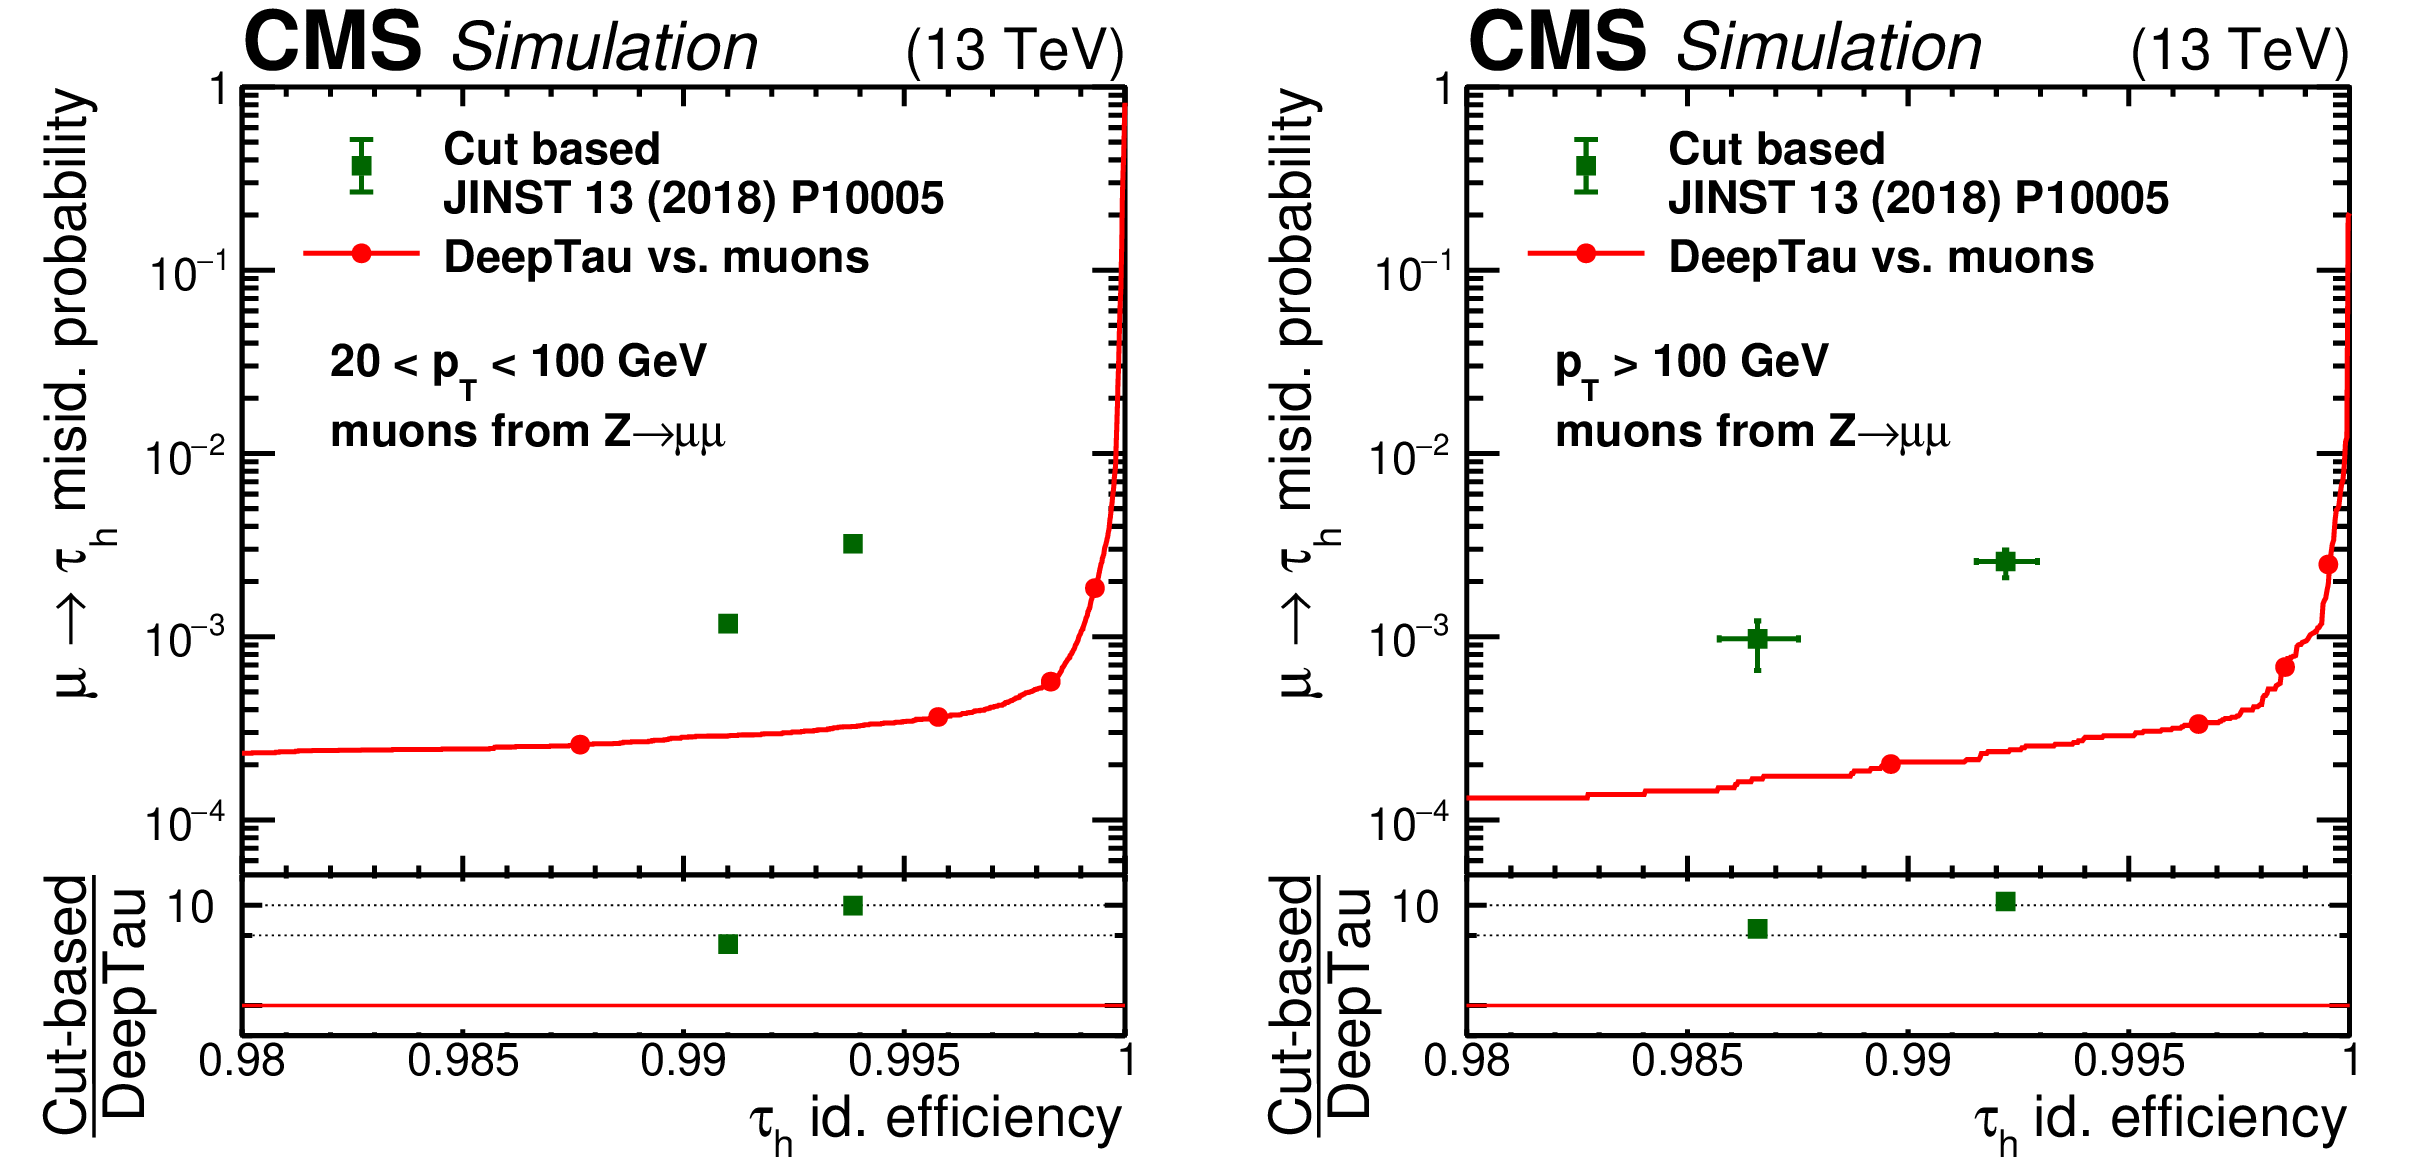
\includegraphics[scale=0.13]{Chapitre4/Images/DeepTauvsMu.png}
        \caption{}
    \end{subfigure}
    \caption{Probabilité de mauvaise identification d'un jet (a), d'un électron (b) ou d'un muon (c) en tau hadronique pour \textit{DeepTau} (rouge) et autres modes d'identification précedemment utilisés \cite{deeptau}.}
    \label{deeptauperf}
\end{figure}

\subsection{Modélisation du bruit de fond $Z\to\tau\tau$ (\textit{embedding})}
\label{embed}

Chaque mesure réalisée au LHC basée sur l'analyse d'un état final comportant des leptons tau est confrontée à un important bruit de fond provenant des désintégrations $Z\rightarrow\tau\tau$. Dans cette optique, une méthode visant à intégrer une paire de leptons tau simulés au sein d'évènements $Z\rightarrow\mu\mu$ collectés par le détecteur CMS dans des collisions proton-proton a été mise au point \cite{Embedding}, et est notamment utilisée dans l'analyse des propriétés CP du boson de Higgs présentée dans cette thèse. Cette méthode permet de s'affranchir des difficultés de simulation de l'empilement et des gerbes hadroniques produites conjointement dans ce type d'évènement en offrant des échantillons de données hybrides dans lesquels seuls les leptons tau sont simulés. \\ 


\begin{figure}
\centering
    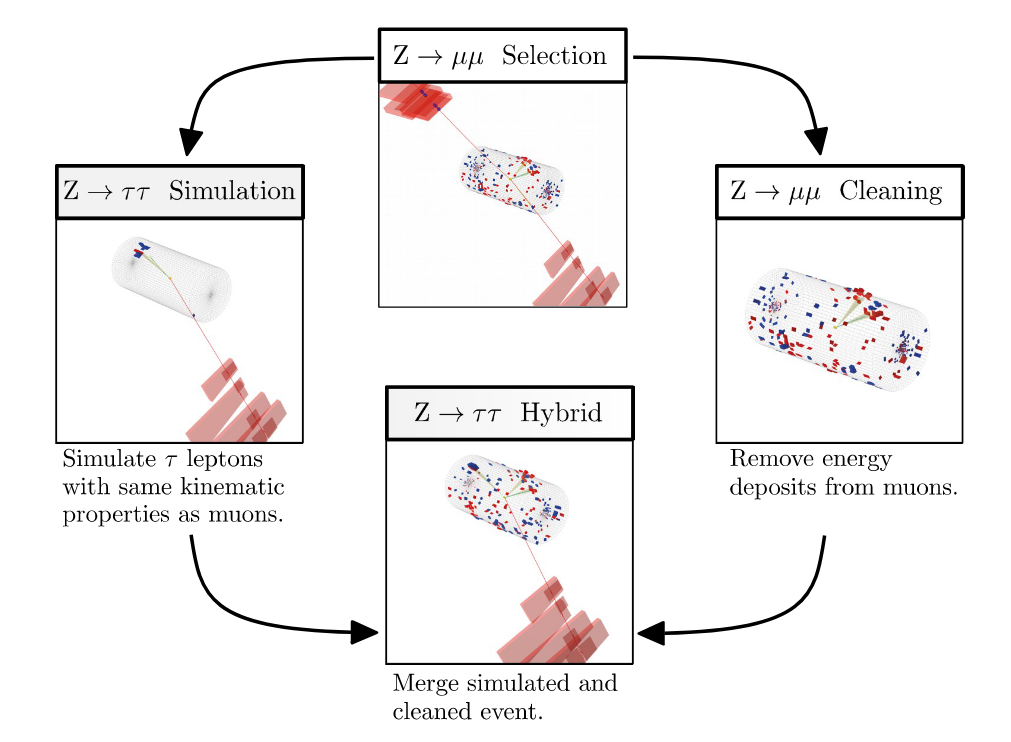
\includegraphics[scale=0.38]{Chapitre4/Images/4steps.png} 
    \caption{Intégration d'une paire de leptons tau simulés dans un évènement $Z\rightarrow\mu\mu$ en 4 étapes : sélection (\textit{selection}), simulation (\textit{simulation}), nettoyage (\textit{cleaning}), regroupement (\textit{merging}) \cite{Embedding}.}
    \label{4steps}
\end{figure} 

La méthode d'intégration des leptons tau, appelée couramment $\textit{"embedding"}$, repose majoritairement sur l'hypothèse de l'universalité leptonique. Cette dernière stipule que les trois saveurs leptoniques sont équivalentes face au couplage faible, permettant de garantir qu'une désintégration $Z\rightarrow\tau\tau$ se déroulera dans un environnement sous-jacent parfaitement identique à celui d'une désintégration $Z\rightarrow\mu\mu$ et avec la même probabilité. En tenant aussi compte de l'excellente performance du détecteur CMS dans l'identification et la reconstruction des muons, il est alors possible de concevoir une méthode dans laquelle des évènements $Z\rightarrow\mu\mu$ sont utilisés afin d'y intégrer une paire de leptons tau simulés avec les mêmes propriétés cinématiques. La production d'un évènement hybride se déroule selon quatre étapes majeures décrites ci-dessous et résumées dans la figure \ref{4steps} :

\begin{enumerate}
    \medskip
    \item \textbf{Sélection} d'un évènement $Z\rightarrow\mu\mu$ dans les données.
    \medskip
    \item \textbf{Simulation} d'une paire de leptons tau avec des propriétés cinématiques équivalentes aux muons précédemment identifiés.
    \medskip
    \item \textbf{Nettoyage} des traces et des dépôts d'énergie des muons de l'évènement sélectionné.
    \medskip
    \item \textbf{Regroupement} de l'évènement nettoyé et de la paire simulée.
    \medskip
\end{enumerate}

Ce type d'échantillon est d'un intérêt particulier dans les analyses impliquant des désintégrations $Z\rightarrow\tau\tau$ puisqu'elle offre une meilleure description des données que les échantillons purement simulés. La figure \ref{embedindata} présente la distribution de quelques variables dans l'état final $\mu\tau_h$ ainsi que l'accord entre données et simulation dans les données de 2017. On remarque une amélioration globale de cet accord lorsque la contribution des évènements $Z\rightarrow\tau\tau$ est estimée grâce à \textit{l'embedding}. La section \ref{optvar} est dédiée à une étude des variables optimales de spin du lepton tau dans ces échantillons.  \\
\vskip 1cm
\begin{figure}[!ht]
  \begin{subfigure}[b]{0.33\linewidth}
    \centering
    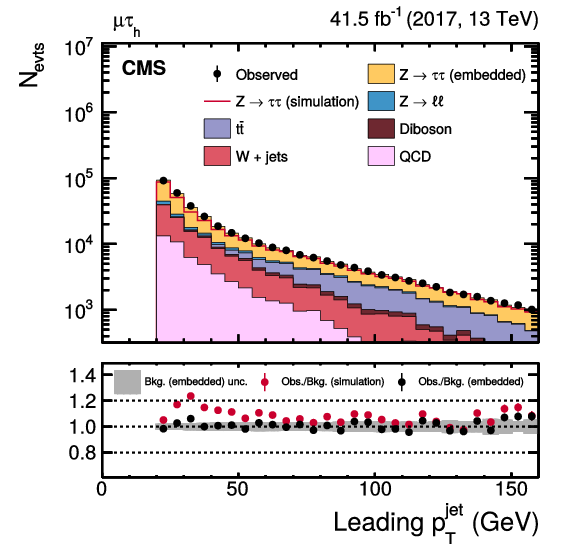
\includegraphics[width=\linewidth]{Chapitre4/Images/leadj_embed.png} 
    \caption*{} 
    \vspace{0.5ex}
  \end{subfigure}%% 
  \begin{subfigure}[b]{0.33\linewidth}
    \centering
    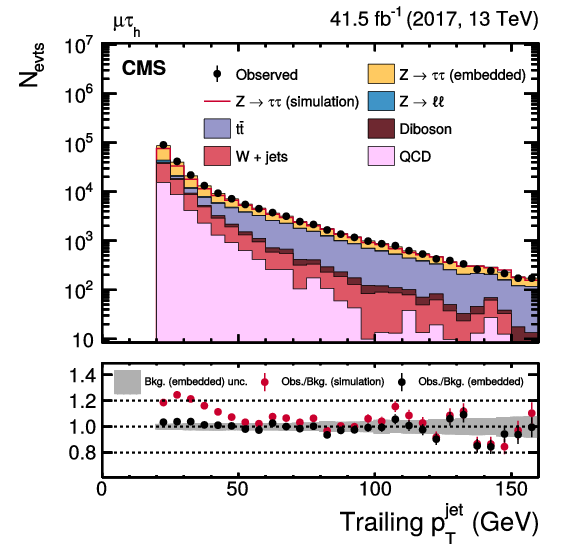
\includegraphics[width=\linewidth]{Chapitre4/Images/trailj_embed.png} 
    \caption*{} 
    \vspace{0.5ex}
  \end{subfigure} 
    \begin{subfigure}[b]{0.33\linewidth}
    \centering
    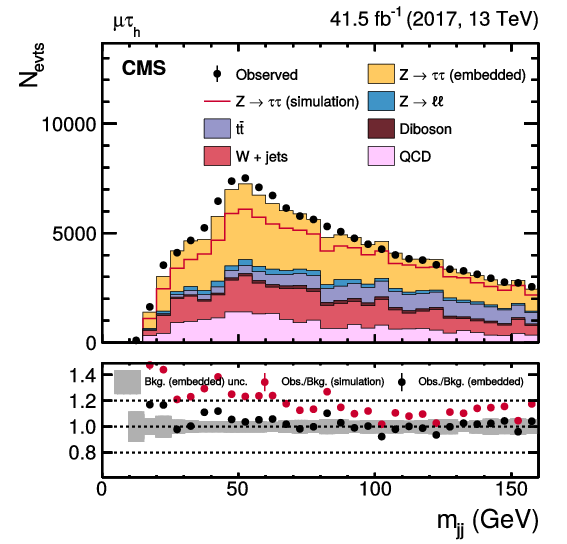
\includegraphics[width=\linewidth]{Chapitre4/Images/mjj_embed.png} 
    \caption*{} 
    \vspace{0.5ex}
  \end{subfigure} 

  \begin{subfigure}[b]{0.33\linewidth}
    \centering
    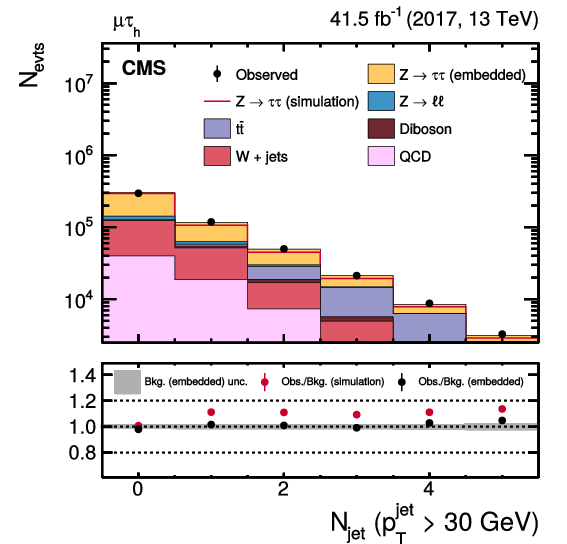
\includegraphics[width=\linewidth]{Chapitre4/Images/Njets_embed.png} 
    \caption*{} 
    \vspace{0.5ex}
  \end{subfigure}%% 
  \begin{subfigure}[b]{0.33\linewidth}
    \centering
    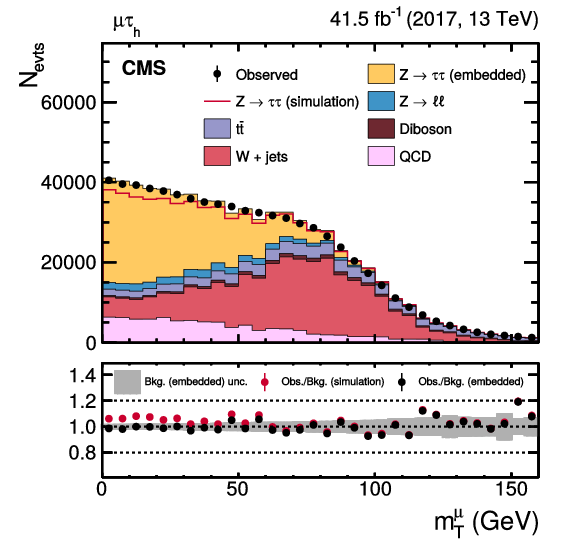
\includegraphics[width=\linewidth]{Chapitre4/Images/mtmu_embed.png} 
    \caption*{} 
    \vspace{0.5ex}
  \end{subfigure} 
    \begin{subfigure}[b]{0.33\linewidth}
    \centering
    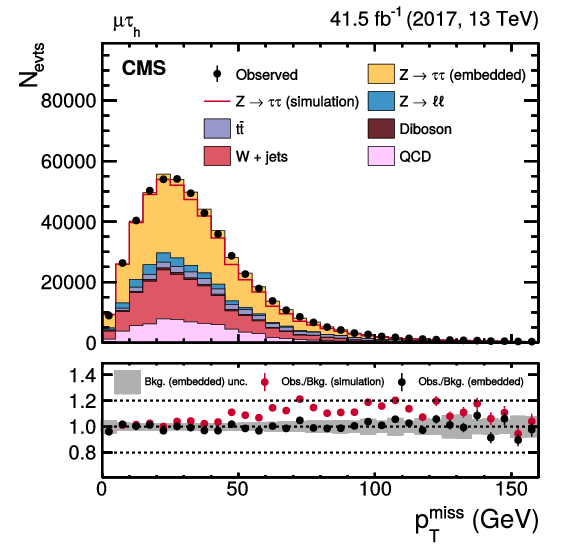
\includegraphics[width=\linewidth]{Chapitre4/Images/ptmiss_embed.png} 
    \caption*{} 
    \vspace{0.5ex}
  \end{subfigure} 
  \caption{Distribution de $p_T$ du jet de plus haute impulsion transverse (haut, gauche), $p_T$ du second jet de plus haute impulsion transverse (haut, centre), $m_{inv}$ de la paire de jets de plus haute impulsion transverse (haut, droite), $N_{jets}$ (bas, gauche), $m_T^{\mu}$ (bas, centre), $p_T^{miss}$ (bas, droite) dans l'état final $\mu\tau_h$. L'estimation de la contribution des évènements $Z\rightarrow\tau\tau$ issus des échantillons Monte Carlo est représentée par la ligne rouge \cite{Embedding}.}
  \label{embedindata}
\end{figure}
\clearpage
\section{Impact de l'identification des électrons et photons sur la reconstruction des leptons tau}

Une étude des performances de l'algorithme HPS a été réalisée au cours de cette thèse dans le cadre des EPR afin de mesurer l'impact de l'identification des électrons et des photons reconstruits par le flux de particules sur la reconstruction des leptons tau. Lors du démarrage du Run 2, une perte d'efficacité de reconstruction du mode de désintégration $\tau_h\rightarrow\pi^{\pm}+\pi^0s$ (DM1+DM2) de l'ordre de $5-10\%$ en comparaison avec les performances du Run 1 fut observée. Cette perte est attribuée au déploiement d'une nouvelle méthode d'identification des photons s'appuyant sur un réseau de neurone ($e/\gamma$-ID) au cours de laquelle les photons convertis en paire électron/positron peuvent être reconstruits à partir d'une seule trace lorsque la seconde est perdue (\textit{single-track photon conversions}). Lors de cette identification, plusieurs éléments tels que les traces ou dépôts d'énergie de hadrons ($\pi^{\pm},\pi^0$) peuvent être faussement associés à des photons, tandis qu'un effet similaire mais réduit est observé pour le mode de désintégration $\tau_h\rightarrow\pi^{\pm}$ (DM0). Cette étude permet d'évaluer les performances du $e/\gamma$-ID, ré-entraîné en prévision du Run 3, et de s'assurer que son utilisation n'entraîne pas de perte de performance supplémentaire dans l'identification des leptons tau. \\

\begin{figure}[!ht]
\captionsetup{justification=centering}
  \begin{subfigure}{0.5\linewidth}
    \centering
    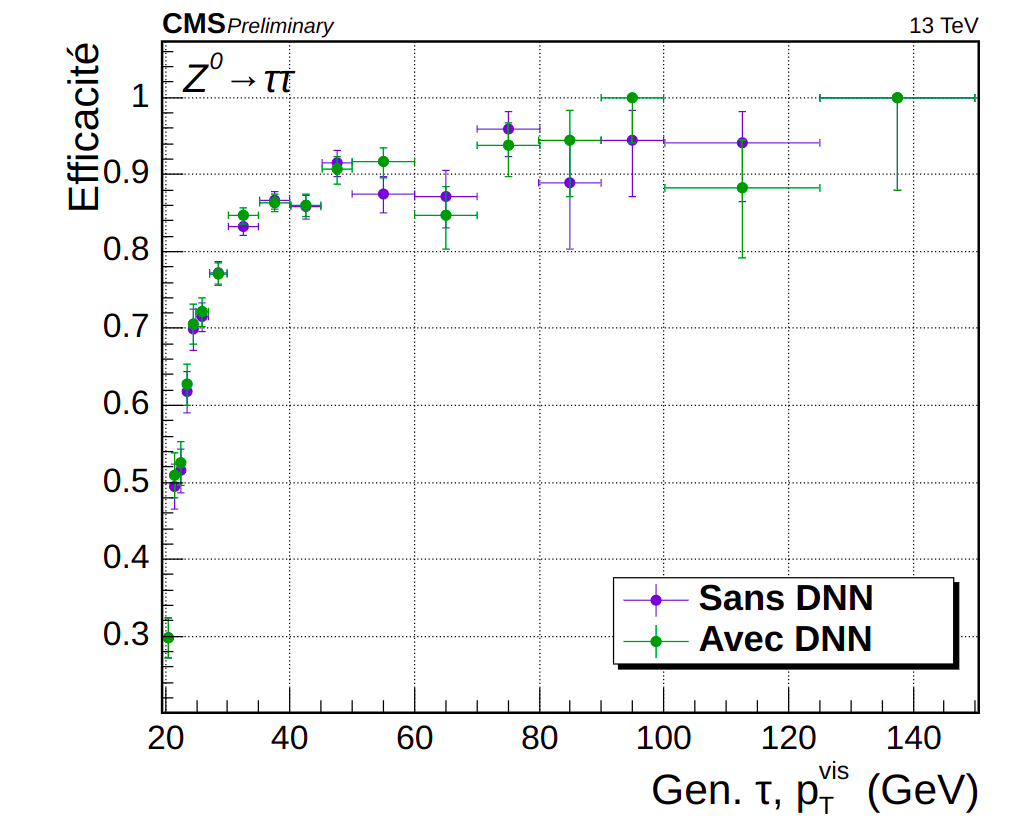
\includegraphics[width=0.8\linewidth]{Chapitre4/Images/HPSnewDMs_ztt_pt.png} 
    \caption{Efficacité vs $p_T^{\text{vis}}$ dans l'échantillon \\ $Z\rightarrow\tau\tau$} 
  \end{subfigure}
  \begin{subfigure}{0.5\linewidth}
    \centering
    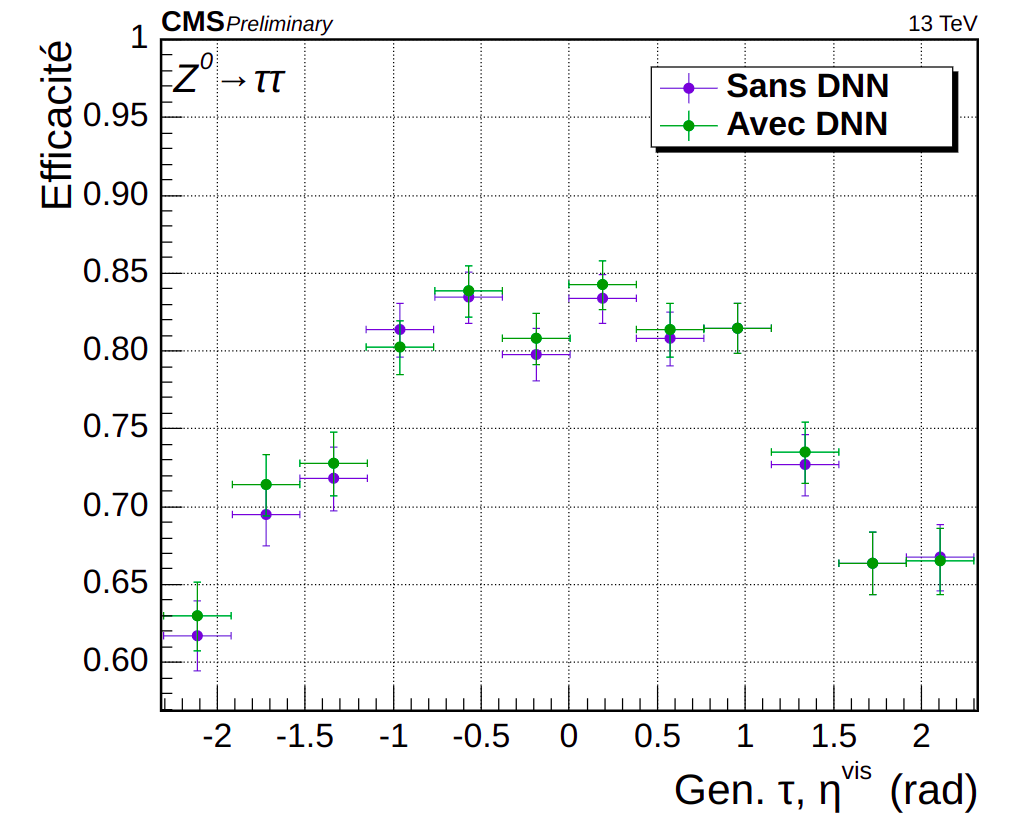
\includegraphics[width=0.8\linewidth]{Chapitre4/Images/HPSnewDMs_ztt_eta.png} 
    \caption{Efficacité vs $\eta^{\text{vis}}$ dans l'échantillon \\ $Z\rightarrow\tau\tau$} 
  \end{subfigure} 
  \begin{subfigure}{0.5\linewidth}
    \centering
    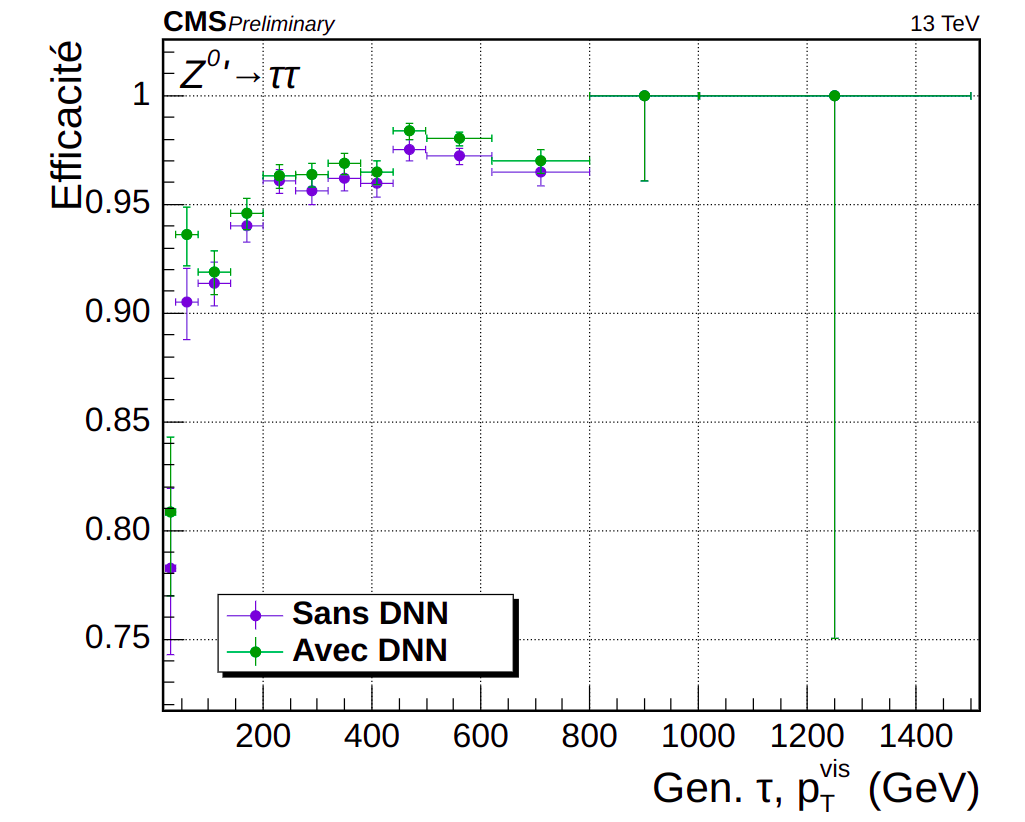
\includegraphics[width=0.8\linewidth]{Chapitre4/Images/HPSnewDMs_zptt_pt.png} 
    \caption{Efficacité vs $p_T^{\text{vis}}$ dans l'échantillon \\ $Z'\rightarrow\tau\tau$} 
  \end{subfigure}
  \begin{subfigure}{0.5\linewidth}
    \centering
    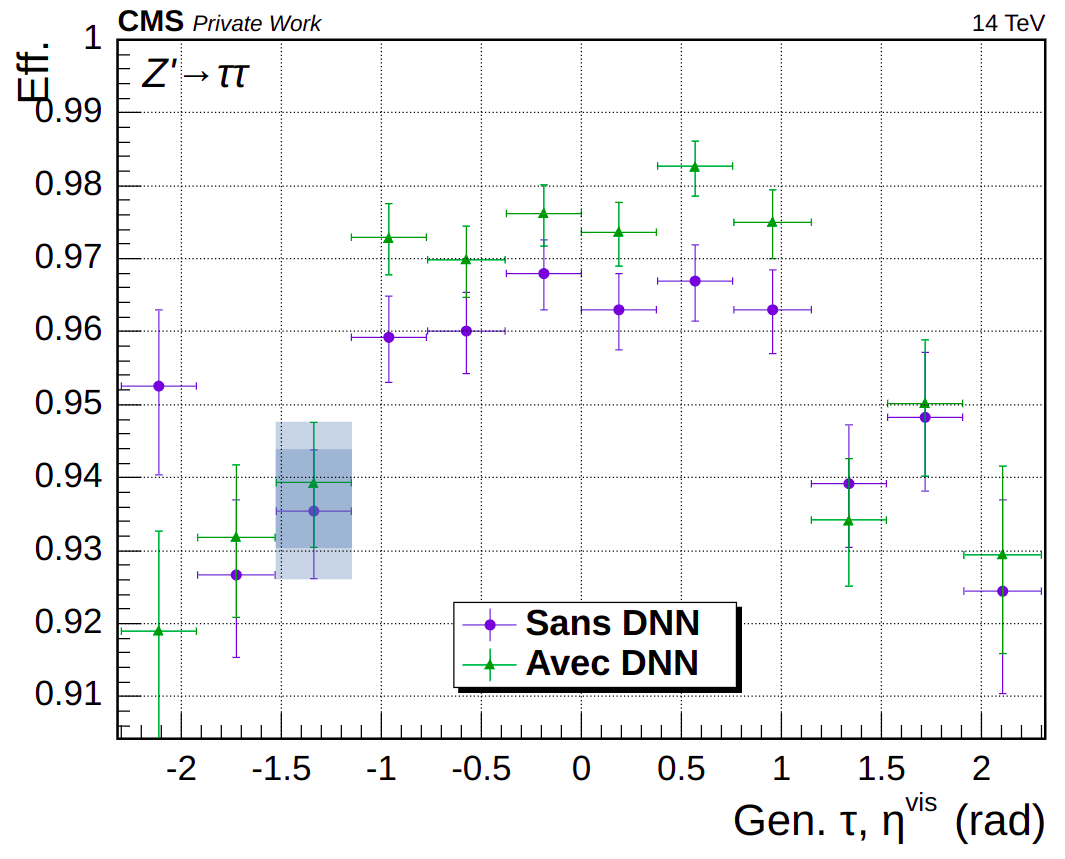
\includegraphics[width=0.8\linewidth]{Chapitre4/Images/HPSnewDMs_zptt_eta.png} 
    \caption{Efficacité vs $\eta^{\text{vis}}$ dans l'échantillon \\ $Z'\rightarrow\tau\tau$} 
  \end{subfigure}
  \begin{subfigure}{0.5\linewidth}
    \centering
    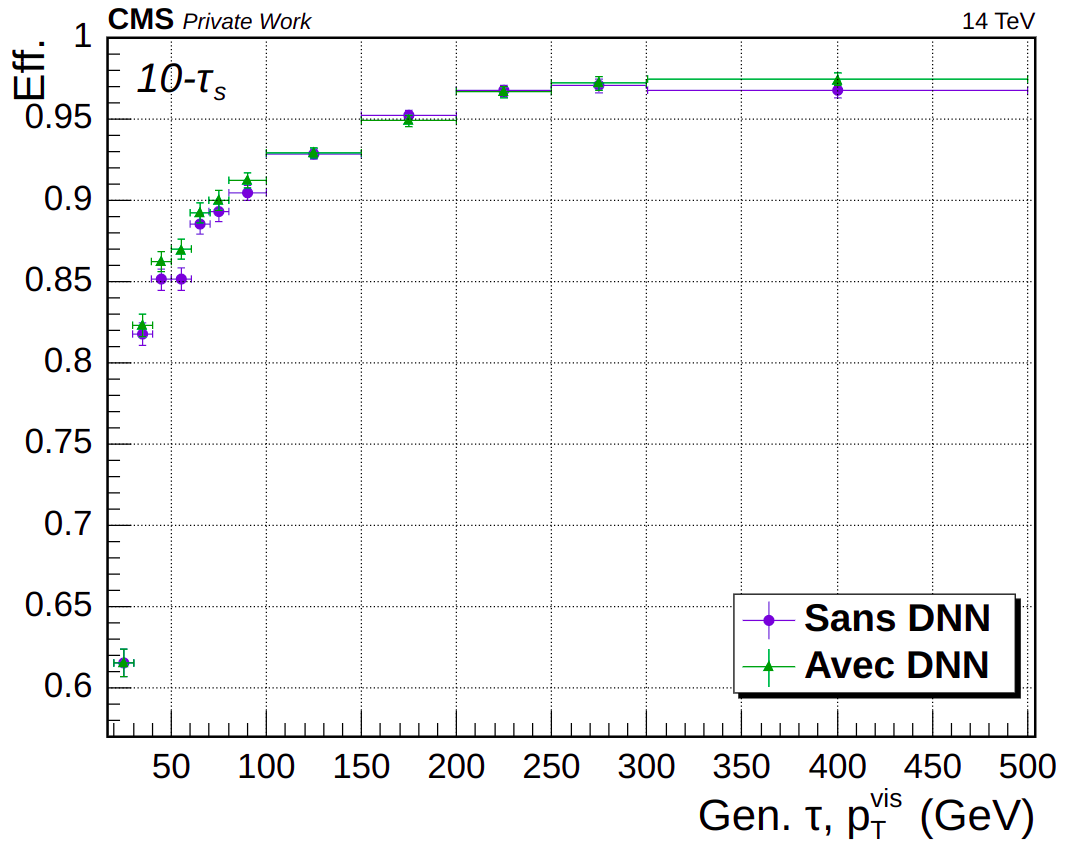
\includegraphics[width=0.8\linewidth]{Chapitre4/Images/HPSnewDMs_10t_pt.png} 
    \caption{Efficacité vs $p_T^{\text{vis}}$ dans l'échantillon \\ "\textit{TauGun}"} 
  \end{subfigure}
  \begin{subfigure}{0.5\linewidth}
    \centering
    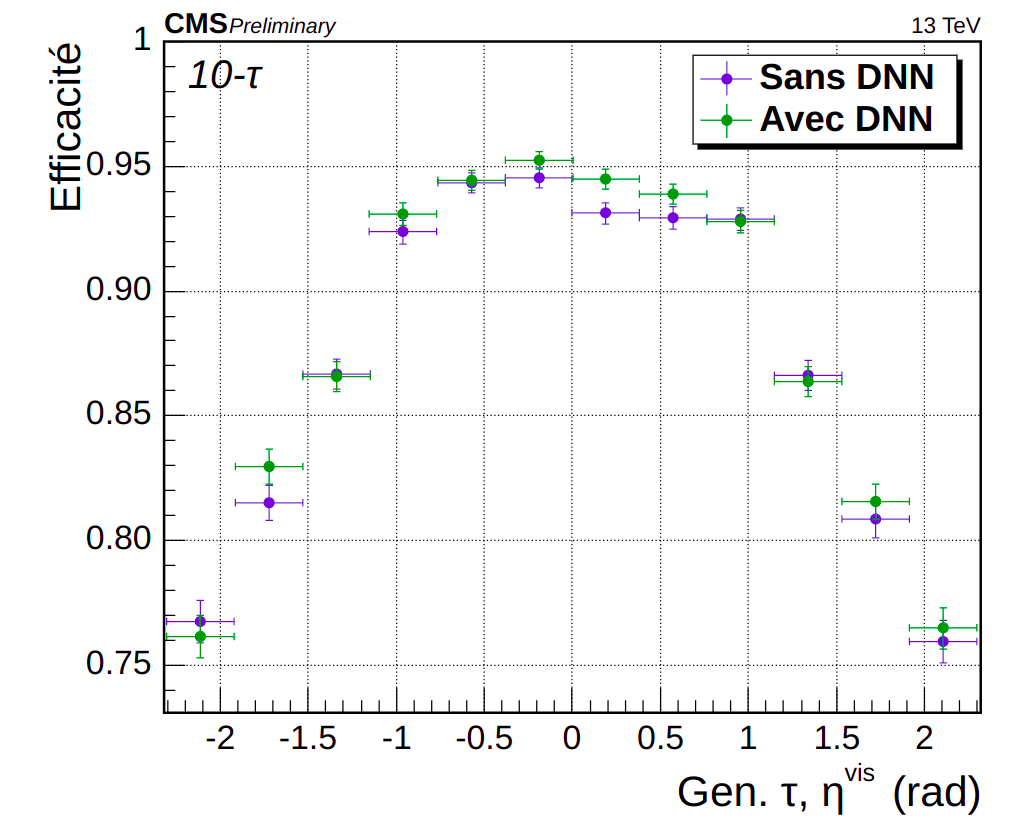
\includegraphics[width=0.8\linewidth]{Chapitre4/Images/HPSnewDMs_10t_eta.png} 
    \caption{Efficacité vs $\eta^{\text{vis}}$ dans l'échantillon \\ "\textit{TauGun}"} 
  \end{subfigure} 
  \caption{Efficacité de l'algorithme HPS en fonction de $p_T^{\text{vis}}$ et $\eta^{\text{vis}}$ des leptons tau générés.}
  \label{TenTaus1}
\end{figure}

\begin{figure}[!ht]
  \begin{subfigure}{0.5\linewidth}
    \centering
    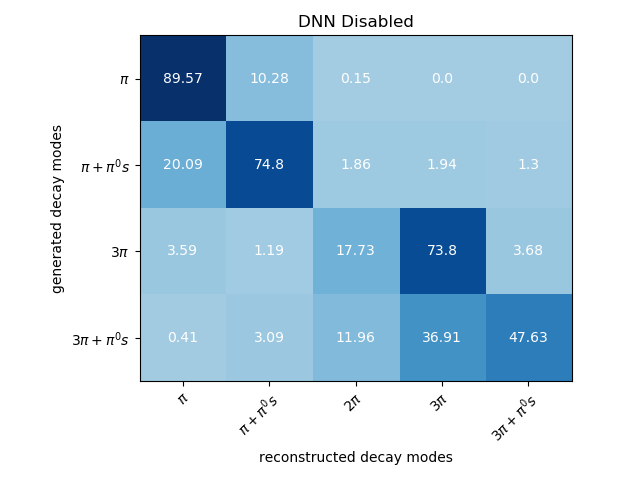
\includegraphics[width=1\linewidth]{Chapitre4/Images/DMmatrices/Matrix_DNNDisabled.png} 
    \caption{Échantillon $Z\rightarrow\tau\tau$, sans DNN.}
    \vspace{0.5ex}
  \end{subfigure}
  \begin{subfigure}{0.5\linewidth}
    \centering
    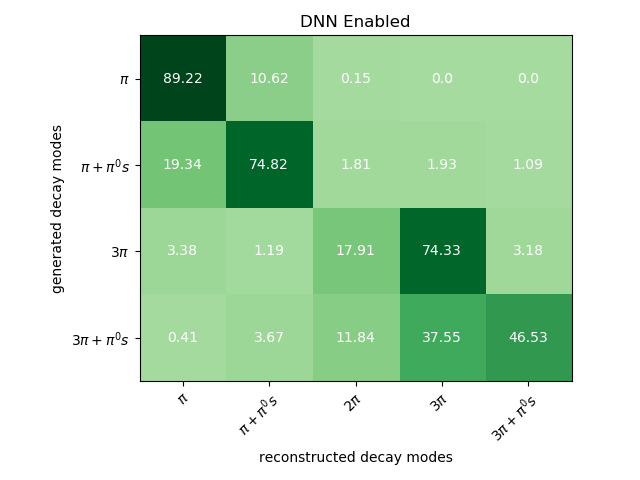
\includegraphics[width=1\linewidth]{Chapitre4/Images/DMmatrices/Matrix_DNNEnabled.png} 
    \caption{Échantillon $Z\rightarrow\tau\tau$, avec DNN.}
    \vspace{0.5ex}
  \end{subfigure} 
  \begin{subfigure}{0.5\linewidth}
    \centering
    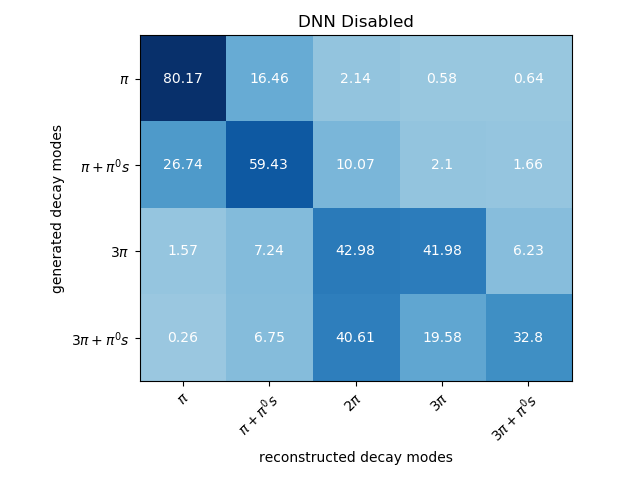
\includegraphics[width=1\linewidth]{Chapitre4/Images/DMmatrices/Matrix_DNNDisabled_ZpTT.png} 
    \caption{Échantillon $Z'\rightarrow\tau\tau$, sans DNN.}
    \vspace{0.5ex}
  \end{subfigure}
  \begin{subfigure}{0.5\linewidth}
    \centering
    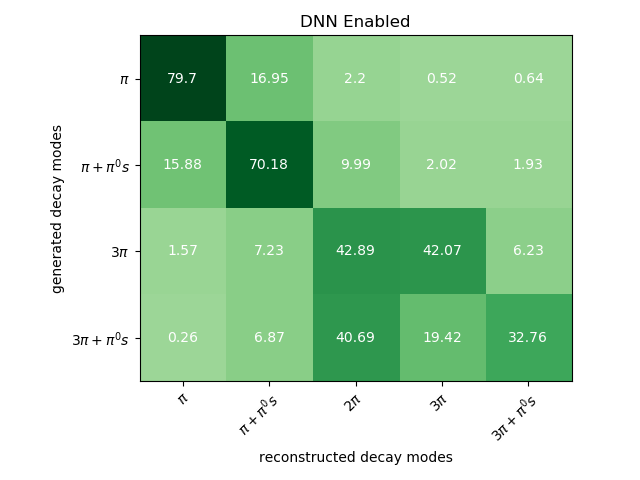
\includegraphics[width=1\linewidth]{Chapitre4/Images/DMmatrices/Matrix_DNNEnabled_ZpTT.png} 
    \caption{Échantillon $Z'\rightarrow\tau\tau$, avec DNN.}
    \vspace{0.5ex}
  \end{subfigure} 
  \begin{subfigure}{0.5\linewidth}
    \centering
    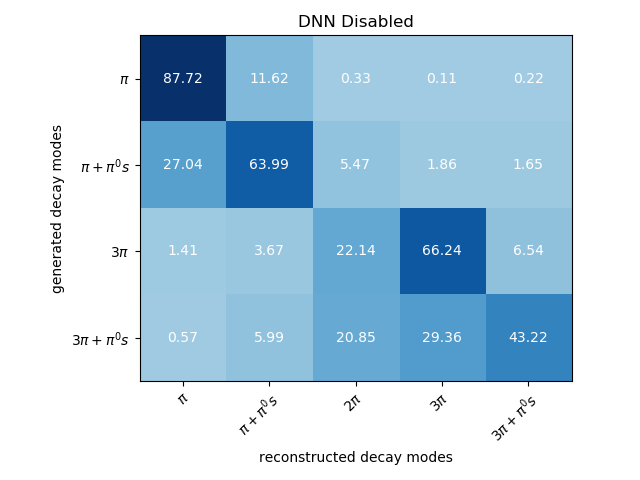
\includegraphics[width=1\linewidth]{Chapitre4/Images/DMmatrices/Matrix_DNNDisabled_10taus.png} 
    \caption{Échantillon "\textit{TauGun}", avec DNN.}
    \vspace{0.5ex}
  \end{subfigure}
  \begin{subfigure}{0.5\linewidth}
    \centering
    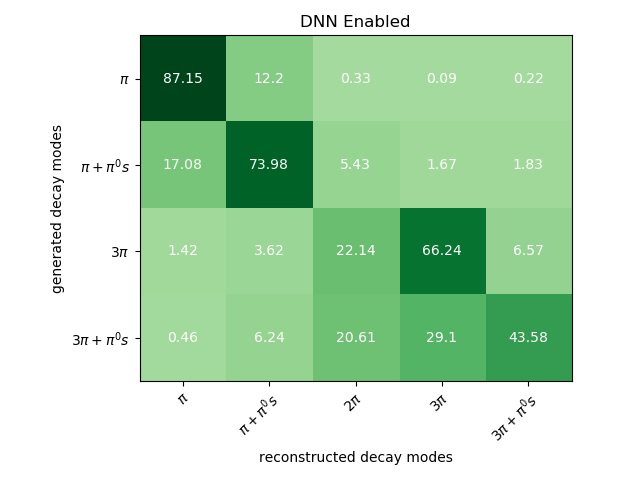
\includegraphics[width=1\linewidth]{Chapitre4/Images/DMmatrices/Matrix_DNNEnabled_10taus.png} 
    \caption{Échantillon "\textit{TauGun}", sans DNN.}
    \vspace{0.5ex}
  \end{subfigure} 
  \caption{Matrices de confusion des modes de désintégration HPS normalisées par lignes.}
  \label{DMmatrix}
\end{figure}

Trois échantillons de données simulés ont été utilisés pour cette étude : un premier comportant des évènements $Z\rightarrow\tau\tau$ tels que décrits par le modèle standard produits dans des collisions $pp$ à $\sqrt{s}=14$ TeV avec des leptons tau couvrant une plage d'impulsion transverse allant de $20$ à $150$ GeV, un second analogue avec un boson $Z'$ plus lourd permettant de couvrir une plage d'impulsion transverse atteignant $1500$ GeV et enfin un sample "\textit{TauGun}" dans lequel des leptons taus sont simulés uniformément avec une impulsion transverse variant de $15$ à $500$ GeV à raison de dix leptons tau par évènement. La figure \ref{TenTaus1} présentent la distribution de l'efficacité de l'algorithme HPS en fonction de l'impulsion transverse et de la coordonné $\eta$ de la partie visible des taus simulés dans les trois échantillons. Dans ce cadre, l'efficacité est définie comme la proportion de taus reconstruits avec un mode de désintégration correctement attribué ou non. Ces distributions montrent que l'efficacité de reconstruction des leptons tau obtenue avec le $e/\gamma$-ID est compatible avec celle lorsque ce dernier n'est pas employé et que le nouvel entraînement ne provoque pas de perte d'efficacité supplémentaire. La figure \ref{DMmatrix} montre les matrices de confusion pour chaque modes de désintégration normalisées par lignes. La pureté des modes désintégration $\tau_h\rightarrow\pi^{\pm}+\pi^0s$ (DM1+DM2) est améliorée d'environ $15\%$ dans les échantillons $Z'$ et "\textit{TauGun}". La figure \ref{DM12} montre quant à elle que cette amélioration a en effet principalement lieu à haute impulsion transverse entre $100$ et $200$ GeV, justifiant un effet moindre au sein de l'échantillon $Z\rightarrow\tau\tau$. En conclusion, le nouveau $e/\gamma$-ID présenté offre des performances stables vis à vis de l'identification des leptons tau sans néanmoins recouvrir l'efficacité perdue lors entre le Run 1 et le Run 2. En effet, des \textit{recovery modes} intègrent la possibilité d'obtenir un candidat hadron chargé utilisé dans la reconstruction d'un lepton tau non plus seulement à partir d'un hadron chargé du flux de particules (\textit{PF-charged hadron}), mais également à partir :

\begin{itemize}
    \item[$\bullet$] d'un PF-électron, pouvant être un hadron mal identifié lorsque celui-ci est reconstruit comme un \textit{electron supercluster},
    \item[$\bullet$] d'un PF-muon, pouvant être un hadron mal identifié lorsque celui-ci dépose peu d'énergie dans les calorimètres et/ou crée un dépôt d'énergie dans les chambres à muon,
    \item[$\bullet$] d'une trace lorsque celle-ci est rejetée par l'algorithme du flux de particules pour ses critètes de qualité, ou si elle n'est pas associée à un dépôt dans les calorimètres,
    \item[$\bullet$] d'un PF-neutral hadron (hadron neutre) à haute impulsion transverse lorsque la trace n'est pas reconstruite.
\end{itemize}

La figure \ref{recoverymodes} présente l'efficacité de reconstruction des modes de désintégrations les plus sensibles aux effets de migration et tente de montrer l'impact des \textit{recovery modes} seuls sur l'efficacité dans un échantillon $Z\to\tau\tau$. On remarque alors que la majeure partie de l'amélioration de l'efficacité est due aux \textit{recovery modes} seuls et que le gain apporté par le nouvel entraînement est "caché" dans le gain apporté par les \textit{recovery modes}.

\begin{figure}
  \begin{subfigure}{0.5\linewidth}
    \centering
    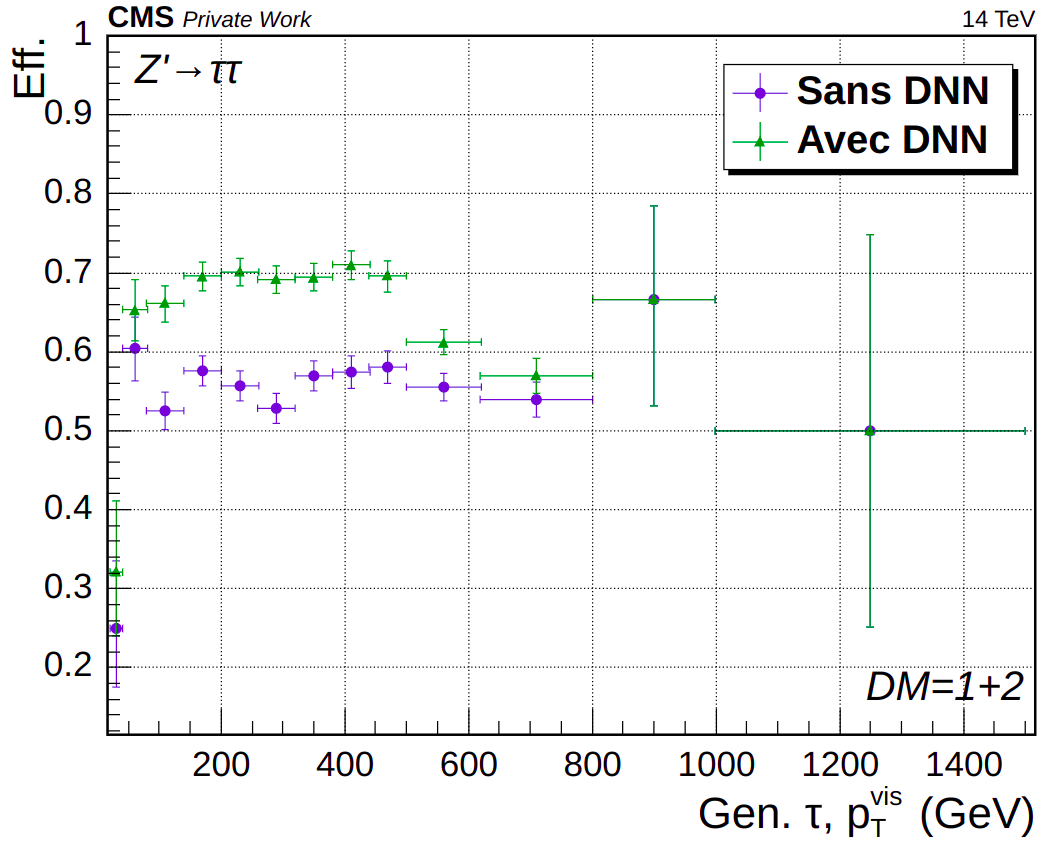
\includegraphics[width=\linewidth]{Chapitre4/Images/HPSnewDM12s_zptt_pt.png} 
  \end{subfigure}
  \begin{subfigure}{0.5\linewidth}
    \centering
    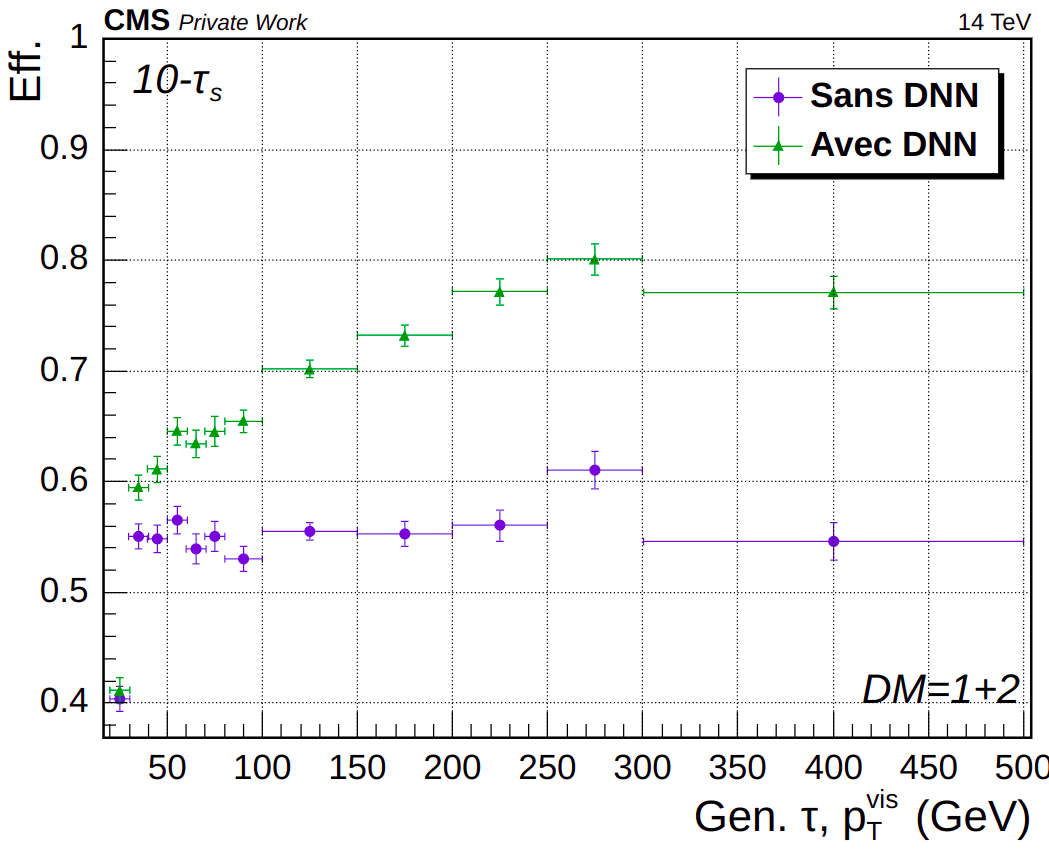
\includegraphics[width=\linewidth]{Chapitre4/Images/HPSnewDM12s_10t_pt.png} 
  \end{subfigure} 
  \caption{Efficacité vs $p_T^{\text{vis}}$ dans l'échantillon $Z'\rightarrow\tau\tau$ (gauche) et "\textit{TauGun}" (droite) pour les modes de désintégration 1 et 2.}
  \label{DM12}
\end{figure}

\begin{figure}[!ht]
    \centering
    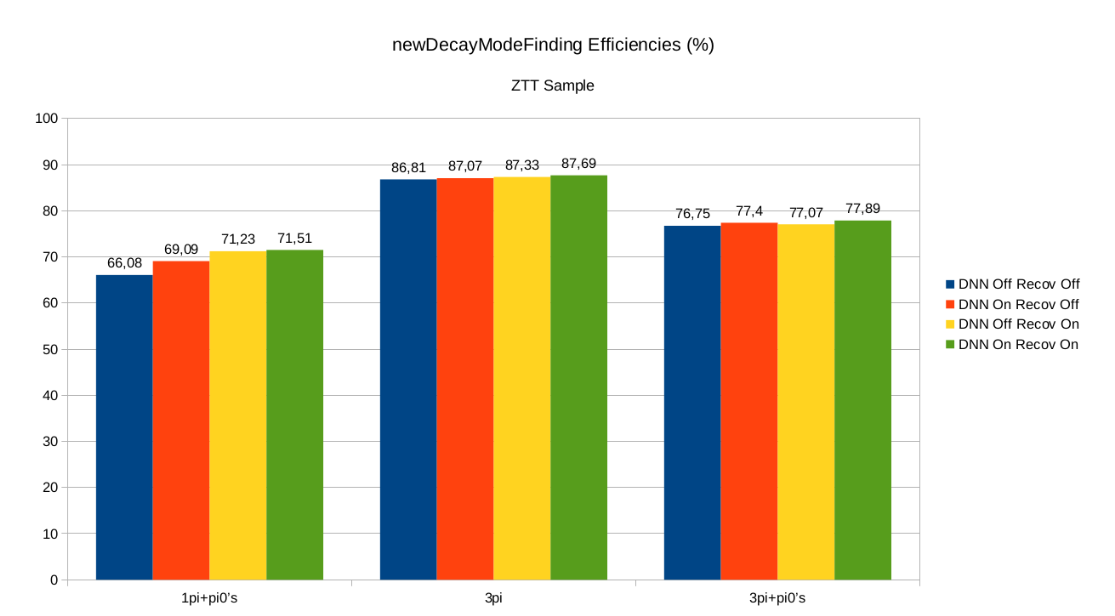
\includegraphics[scale=0.35]{Chapitre4/Images/recov.png} 
  \caption{Efficacité de construction en \% des modes de désintégration $\tau_h\to\pi^{\pm}+\pi^0$s, $\tau_h\to2\pi^{\pm}\pi^{\mp}$, $\tau_h\to2\pi^{\pm}\pi^{\mp}+\pi^0$s sans réseau de neurones et sans recovery modes (bleu), avec réseau de neurones et sans recovery modes (rouge), sans réseau de neurones et avec recovery modes (jaune), avec réseau de neurones et avec recovery modes (vert).}
  \label{recoverymodes}
\end{figure}